\documentclass[12pt, conference]{IEEEtran}
\IEEEoverridecommandlockouts
% The preceding line is only needed to identify funding in the first footnote. If that is unneeded, please comment it out.
\usepackage{cite}
\usepackage{amsmath,amssymb,amsthm,amsfonts}
\usepackage{algorithm2e}
\usepackage{algorithm}
\usepackage{subfigure}
\usepackage{graphicx}
\usepackage{textcomp}
\usepackage{xcolor}
\usepackage{varwidth}
\usepackage{bookmark}
\usepackage[]{hyperref}
\hypersetup{
  bookmarks=true,
  bookmarksnumbered=true,     
  bookmarksopen=true,  
  colorlinks=false , 
  citecolor=.,   
  allbordercolors={white},               
  pdfstartview=Fit,           
  pdfpagemode=UseOutlines
}

  
  
\def\BibTeX{{\rm B\kern-.05em{\sc i\kern-.025em b}\kern-.08em
    T\kern-.1667em\lower.7ex\hbox{E}\kern-.125emX}}
\begin{document}

\title{WiFi Fingerprint Indoor Positioning System}

\author{\IEEEauthorblockN{Braxton Adams\textsuperscript{1}, Cyrus Cravens\textsuperscript{2}, Jonathan Adiri\textsuperscript{3}, Sang Xing\textsuperscript{4}}
  \IEEEauthorblockA{\textit{Department of Mathematics and Statistics}}
  {Portland State University, Portland, OR 97201 USA} \\
  \textsuperscript{1}braadams@pdx.edu, \textsuperscript{2}ccravens@pdx.edu, \textsuperscript{3}adiri@pdx.edu, \textsuperscript{4}sxing@pdx.edu
}

\maketitle



%------------------------------------------------------------------------------------------------------------------------------------
% Abstract and Keywords
%------------------------------------------------------------------------------------------------------------------------------------
\begin{abstract}
If Global Positioning System (GPS) radios are insufficient or infeasible for physically locating a network-connected device, utilizing the network connection itself for an "Indoor Positioning System" is a viable alternative. This paper considers how to use received signal strength indication values to estimate an object's position by using either (1) predicted distances from a linear model as the basis for a trilateration algorithm or (2) by classifying a location based on a k-nearest neighbors (KNN) supervised learning algorithm. The paper finds that the KNN approach provides a higher accuracy than the trilateration method for a given dataset of a floor in a university building.
\end{abstract}

\begin{IEEEkeywords}
  WiFi fingerprinting, WiFi indoor positioning, Trilateration, K-nearest neighbor algorithm
\end{IEEEkeywords}


%------------------------------------------------------------------------------------------------------------------------------------
% Introduction
%------------------------------------------------------------------------------------------------------------------------------------
\section{Introduction}
In recent years, with the ubiquity of mobile and Internet of Things devices, the possibility of creating an Indoor Positioning System (IPS), has become a reality for many structures \cite{b1}. Our client, the engineering department of a university, has requested our team to create a model that predicts the physical location of a device, based on a set of signal strengths between access points and connected devices. The client also asked our team to quantify the accuracy and precision of the model. In order to find the most accurate way of predicting the location, two approaches were adopted in this experiment, The first, Trilateration Technique, is the use of distances for determining the coordinates of a point in space. Since this approach is being used for geopositioning, we thought that it might be applied to IPS as well. The second approach, K-Nearest Neighbor (KNN) method, is a supervised lazy learning algorithm. This approach seems promising because it has been proven successful in the past in solving similar problems.

The client requested that we identify the physical location of devices that are connected to the university network. There are six access points (i.e. wifi routers), with distinct MAC addresses, on a certain floor of one of the university buildings. The floor-plan is roughly 35 by 14 meters and is composed of several classrooms and hallways. Devices that are connected to the network can measure the Received Signal Strength Indication (RSSI) of all access points within range. To collect the data, a mobile device connected to the network has recorded different values at various locations and oriented in various directions. The collected data was split into Offline and Online data, which will later be used to train and test the models developed by our team.
Two approaches were tried. The first method we will introduce is trilateration which is a method for determining the relative position of points by measuring absolute distances to determine the coordinates of a point in space \cite{b2}. Since this approach is being used for geopositioning, we thought that it might be applied to IPS as well. The second approach, KNN, is a non-parametric supervised learning method. This approach seems promising because it has been proven successful in the past at solving similar problems and is a popular approach regarding clustering \cite{b3}.


%------------------------------------------------------------------------------------------------------------------------------------
% Data
%------------------------------------------------------------------------------------------------------------------------------------
\section{Data}
Our group was contacted by a local university who collected data from their internet network. The location for the collected data was on a singular floor of the engineering department building. Their problem is they want to be able to predict the physical location of devices that are connected to the network. The client's overall goal is to have a model capable of taking a set of signal strengths from relevant access points and predicting the physical location of that device. Additionally, they want to have the ability to quantify the accuracy and precision of the model. In the interview, our client explained the general layout of the building's floor and provided a base floor plan layout whose dimensions are roughly 35 by 14 meters . This image included the layout of where the floor's room are, the locations for the relevant wireless access points, all 166 recorded locations that depict the offline receiver locations, as well as the locations for the online receiver points. The placement of the access points was particularly interesting because two were on opposite ends of the left side of the floor, two were in classrooms with one being more centrally located, and the others were on the opposite side of the floor closely positioned with clear lines of sight down their respective corridors. This is interesting because each access point, their locations, and groupings all present the opportunity to factor into the processing of the data for developing a model. 

While the client explained that they had viewed the data, they explained that they had not altered the data that they had collected. From their observations we were able to gather that the data contained extra broadcasted data from ad-hoc devices and wireless access points from other floors. Meaning that our team would need to filter the data to only include records relevant to what the client is interested in. The six wireless access points and their locations were included in a text file along with an offline and online dataset to develop potential methods. The offline data was a text file that contained 166 positions with each location having110 records for every 45 degree orientation. Resulting in each offline location having 880 records for a total of 146,080 recorded records. The text file also contained additional information that was not relevant to the data and needed to be filtered out. The online data contained 60 locations that were asymmetrical compared to the offline data grid. 

With the client having already created the offline and online radio maps, the role for our team would be cleaning the data to develop methods for estimating the locations and their accuracy for devices connected to their network. We identified two potential methods for accomplishing our clients' goal after tidying the data by removing unwanted records and creating a better workable format. The first method we wanted to test was a technique known as trilateration or multilateration. The other method we tested is known as the k-nearest neighbors (KNN) algorithm, which is used in machine learning. The KNN algorithm also has several different subclasses that can be used to better fit or evaluate models as needed. These include a deterministic, probabilistic, and proximity based approaches that each have considerations to take into account \cite{b4, b5}. Both methods use a form of fingerprinting to estimate indoor positioning. Additionally, both methods use the offline phase radio map to test their respective methods against the online radio map. In Figure~\ref{fig: Heat Map of 6 APs}, we provide intuitive heat maps to show our RSSI strength at every access point in all orientations from our offline radio map. After reviewing the data and briefly researching the associated topics, our team concluded that R was the best programming language for accomplishing the objectives. A particularly interesting find was coming across a package that was created for Wi-Fi localization \cite{b4}. Because packages can go out of date if it stops being actively maintained, we decided to develop separate methods for addressing our clients needs. 


\begin{figure}[htbp]
  \centering
  \subfigure[00:0f:a3:39:e1:c0]{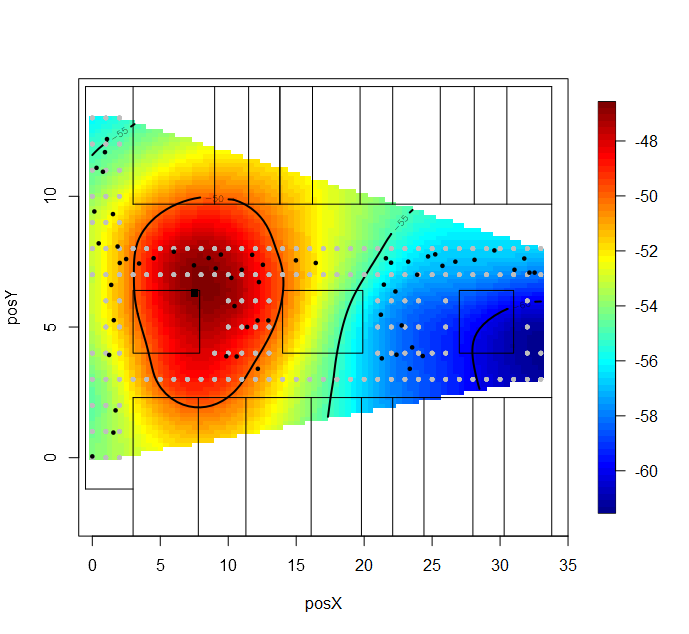
\includegraphics[width=0.24\textwidth]{img/heatMap_allMac_8Angles/Mac-1.png}}
  \subfigure[00:14:bf:b1:97:8a]{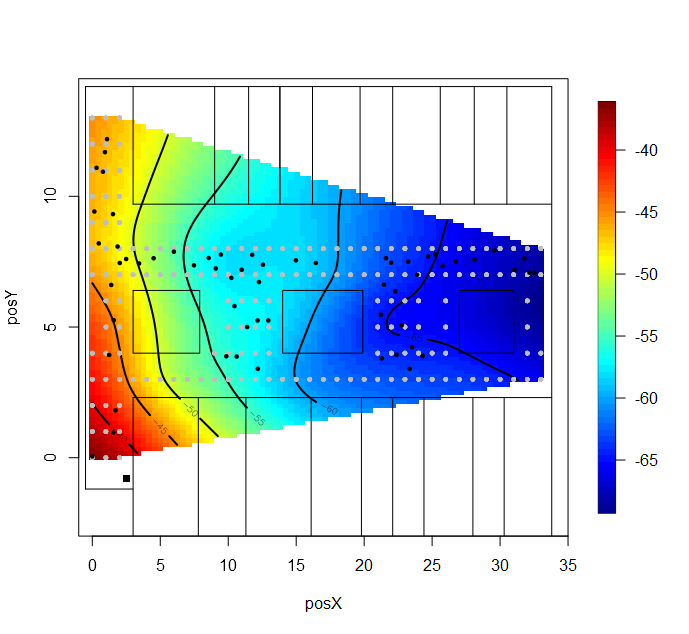
\includegraphics[width=0.24\textwidth]{img/heatMap_allMac_8Angles/Mac-2.png}}
  \subfigure[00:14:bf:3b:c7:c6]{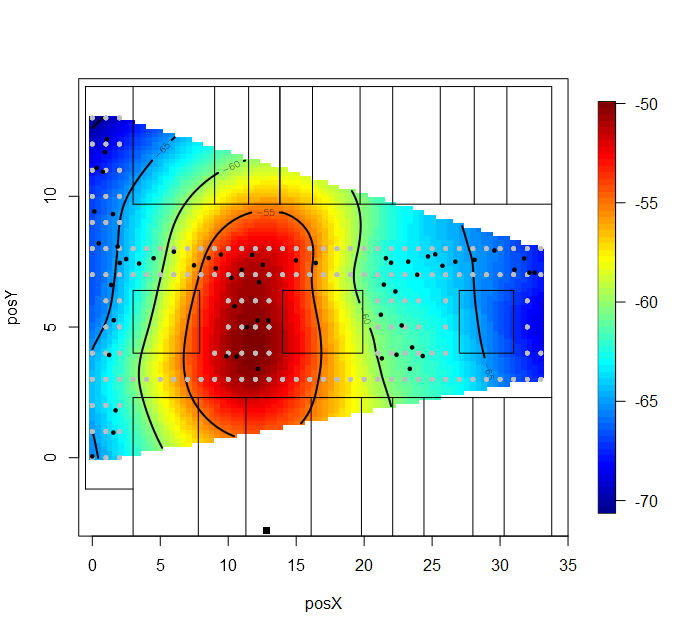
\includegraphics[width=0.24\textwidth]{img/heatMap_allMac_8Angles/Mac-3.png}}
  \subfigure[00:14:bf:b1:97:90]{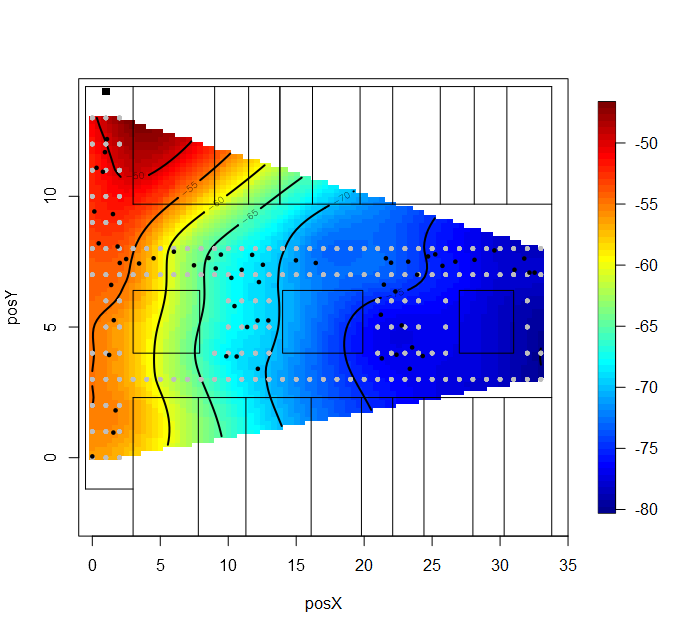
\includegraphics[width=0.24\textwidth]{img/heatMap_allMac_8Angles/Mac-4.png}}
  \subfigure[00:14:bf:b1:97:8d]{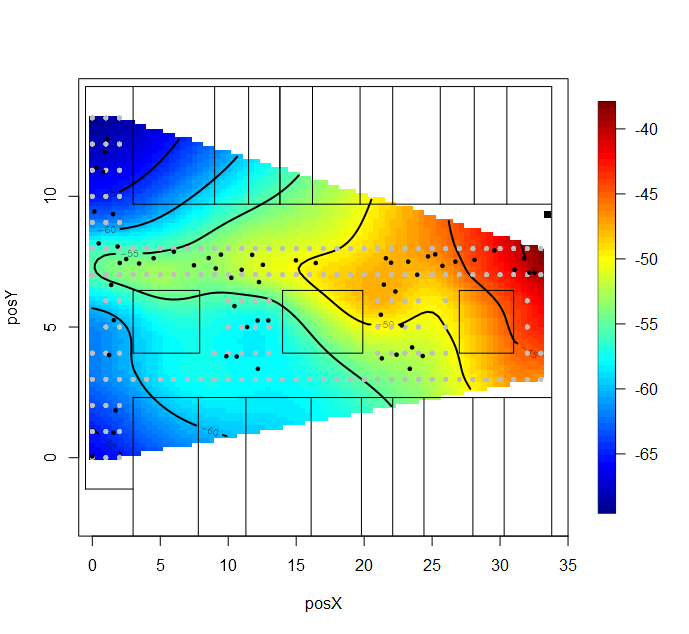
\includegraphics[width=0.24\textwidth]{img/heatMap_allMac_8Angles/Mac-5.png}}
  \subfigure[00:14:bf:b1:97:81]{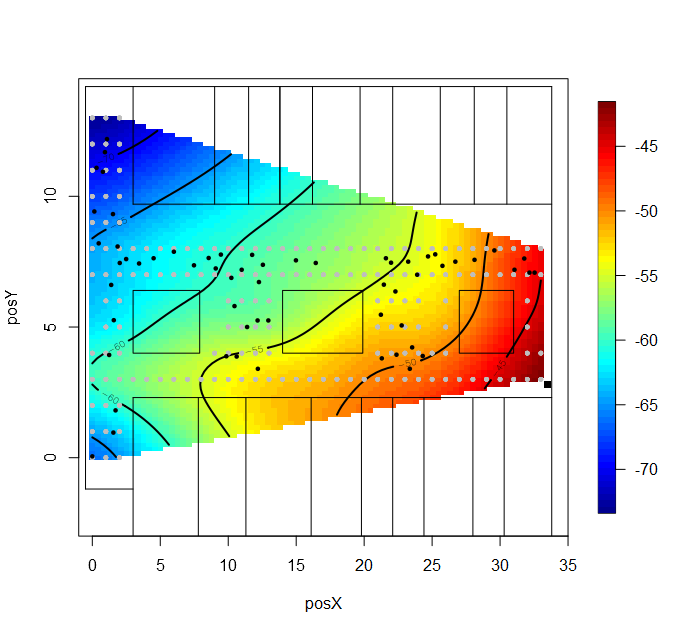
\includegraphics[width=0.24\textwidth]{img/heatMap_allMac_8Angles/Mac-6.png}}
  \caption{Heat map of 6 Access Points in all orientations}
  \label{fig: Heat Map of 6 APs}
\end{figure}


%------------------------------------------------------------------------------------------------------------------------------------
% Methodology
%------------------------------------------------------------------------------------------------------------------------------------
\section{Methodology}

\subsection{Fingerprinting}
Similarly to how governments use fingerprints to identify an individual, indoor positioning uses the fingerprinting method for location. A key to understanding this method is to reflect back on how a government collects peopl'es fingerprints and associates them with other information like social security numbers and dates of birth by creating a database to compare against others. While the chances of two people sharing the same fingerprint is low, it is even smaller when additional variables such as race, date of birth, social security number, associated addresses, or validated pictures are also considered. While indoor position fingerprinting primarily relies on received signal strength indicators (RSSI) values to determine euclidean positioning, these values are closely correlated to other variables similar to government fingerprinting. RSSI values are directly correlated to the wireless access point (WAP) that transmitted the signal to the receiving device known as a receiver. This is accomplished by mapping the RSSI value to the broadcasting access point's media access control (MAC) address which is a unique 12-character alphanumeric attribute that is used to identify individual electronic devices on a network. Additionally, RSSI values are tied to the timestamp in which they are transmitted back to the broadcasting WAP from a receiver. This data is used in conjunction with recorded locations from a receiver to generate what is known as radio maps. Radio maps are typically created in either one or two phases known as offline and online respectively. Similar to how government fingerprint databases use additional variables to identify an individual, Wi-Fi fingerprinting uses RSSI values, MAC addresses, timestamps, and radio maps to create methods for locating devices connected to a network. Fingerprinting is a common strategy used across multiple methods that we will cover in greater detail later in this paper.

\subsection{Trilateration}
Trilateration is a process where the location of an object is determined by measuring the distances to three or more known reference points. This process is utilized in GPS satellite radio navigation and locating earthquake epicenters. However, trilateration works best when the distances are accurately determined; measuring the time that the respective waves take to reach the measuring device is the data of choice for seismology, GPS, and professional WiFi trilateration methods. Our dataset, however, will use signal strength to estimate the distances. Once we have those estimated distances, we will attempt to locate the object by minimizing the sum of squares of the difference between the actual distances and the predicted distances.

When plotting the median signal strength against the distance between the recording point and each access point, we identify that there is a relationship between the distance and signal strength. The heat maps of RSSI values suggest however that this may not be a simple relationship. For example, the access point with the MAC address $\texttt{"00:14:bf:b1:97:8a"}$ has a strong signal strength across the entire left hallway, something that appears as a "shelf" on the corresponding scatter plot.

\begin{figure}[htbp]
  \centerline{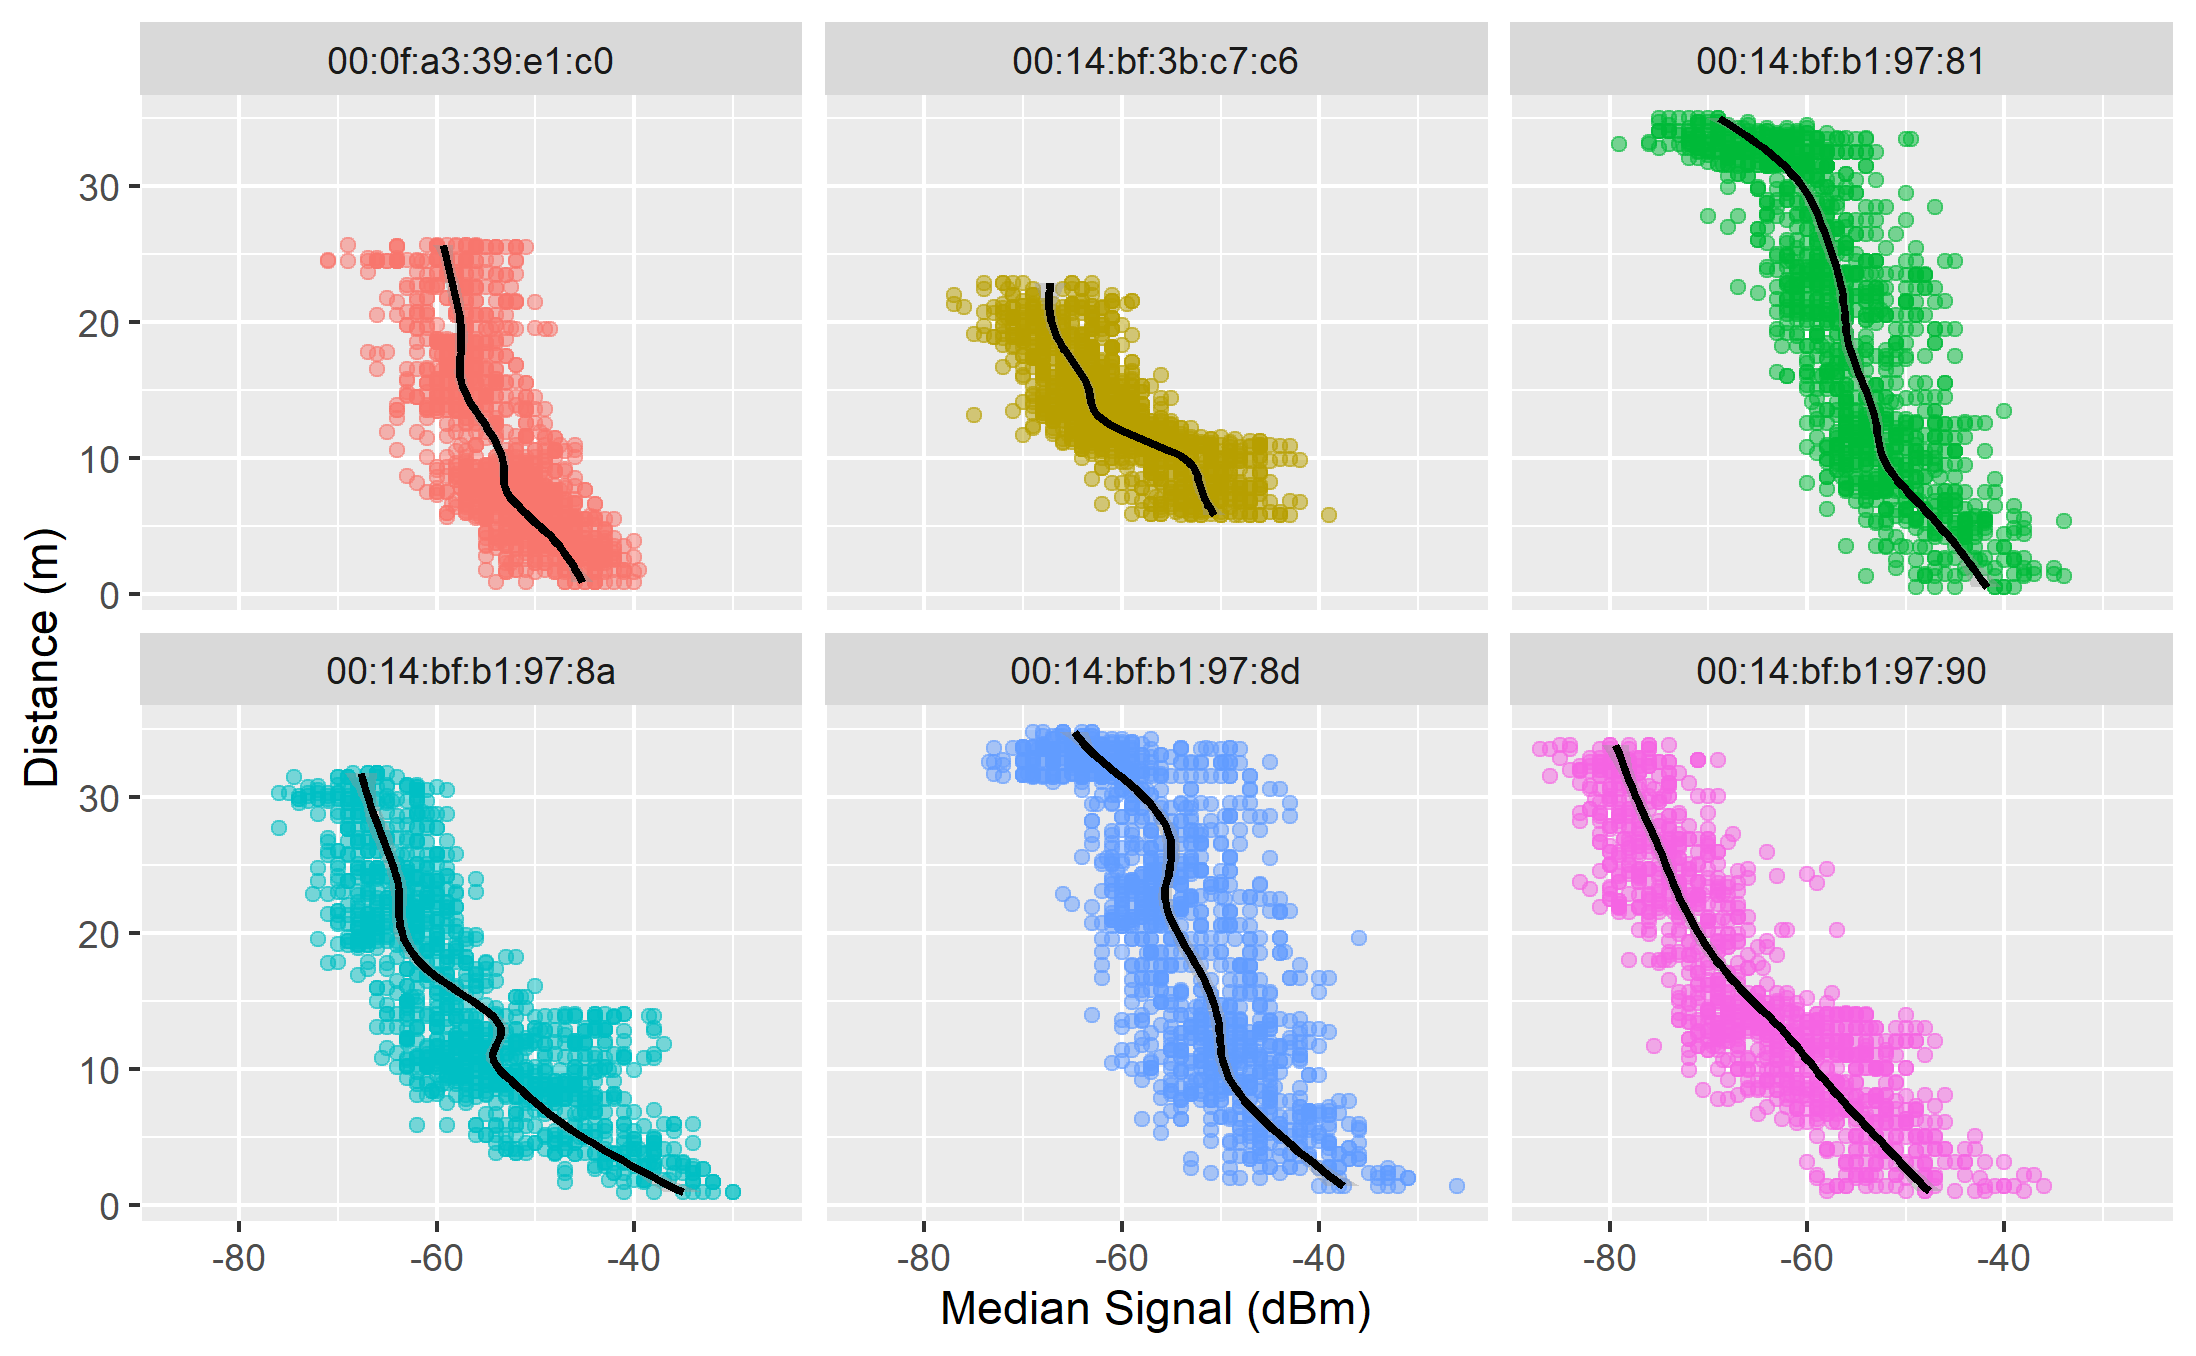
\includegraphics[width=\columnwidth]{img/distance_against_median_signal.png}}
  \caption{Scatterplot of Median Signal Strength against Distance (grouped by access point MAC address)}
  \label{fig: Distance Distribution}
\end{figure}

To model the distances, we will only use the signal strength and the MAC addresses. The orientation of the operator holding the recording device can be shown to impact isolated locations, but the average trend across the entire dataset was unclear and will, for this technique, be dropped. Since the scatter plots shows some nonlinearity in the dataset, we will consider a transformation; using the box-cox method, it was found that the median signal has a more linear relationship with the square root of the distance. Since light follows the inverse square law, this makes sense, though it should be noted that the signal strength being measured in a logarithmic scale (decibel-milliwatts), we should be cautious about how to interpret the square root distance having a better linear relationship than the original distance measurement.

We constructed a separate linear model for each MAC address. Although the end result is identical to a single model that includes the interaction between the signal strength and access point, separating them means we can provide a coefficient of determination ($R^2$) for each linear model to determine which MAC address is easiest to predict the distance for. One way to interpret this is that, for the MAC address \texttt{"00:14:bf:b1:97:8a"}, we can say that $\texttt{67.98\%}$ of the variation in the dataset can be described by our model.

\begin{table}[]
  \centering
  \begin{tabular}{|l|l|}
  \hline
  MAC Address       & $R^2$                \\ \hline
  00:0f:a3:39:e1:c0 & 0.5418               \\ \hline
  00:14:bf:3b:c7:c6 & 0.602                \\ \hline
  00:14:bf:b1:97:81 & 0.6302               \\ \hline
  00:14:bf:b1:97:8a & 0.6798               \\ \hline
  00:14:bf:b1:97:8d & 0.5839               \\ \hline
  00:14:bf:b1:97:90 & 0.7637               \\ \hline
  Full model        & 0.6795               \\ \hline
  \end{tabular} \label{fig: lm_r2}
\end{table}

Once we have our models constructed based off of the offline training dataset, we can then predict the distances between each location in the online validation dataset and each access point. The following chart shows histograms showing the "residuals" or differences between each predicted distance and the actual distance. Note that we are within $\pm 10$ meters regardless of MAC address.

\begin{figure}[htbp]
  \centerline{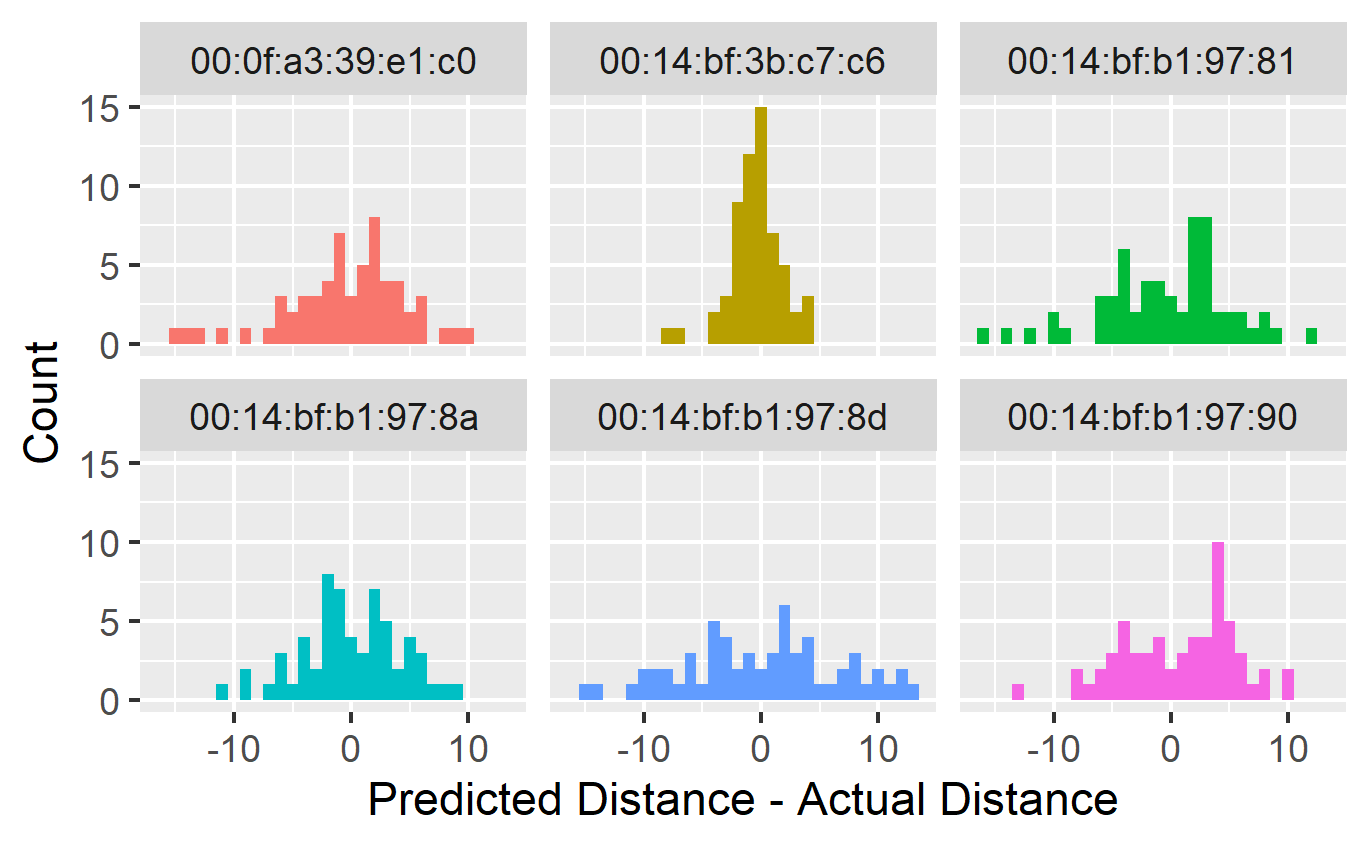
\includegraphics[width=\columnwidth]{img/Distance_error_hist.png}}
  \caption{Histogram of residuals for predicted distance (grouped by access point MAC address)}
  \label{fig: K-Fold CV}
\end{figure}

With these predicted distances, we now can attempt to predict the actual location for each of the locations in the online validation dataset by minimizing the sum of squares error. Starting with an initial guess that is in the center of the building, we measure the actual distances between the guess and each access point, subtract those distances from the predicted distances, square these differences, and then sum the squares. This is the value we wish to minimize.

$$
\min \sum_{i} (\hat{d}_i - d_i)^2
$$

The process is visualized in the below figure for one example data point, the location found at (11.76, 7.76). Note that the circles do not intersect at a single point, which would be the ideal with more accurate distance predictions. This is the primary reason we went with optimizing the least sum of square error, since it provided the simplest way to handle this discrepancy. Future work could utilize picking the centroid of the intersection of each circle, or if no such intersection exists, to increase the size of each circle equally until such.

\begin{figure}[htbp]
  \centerline{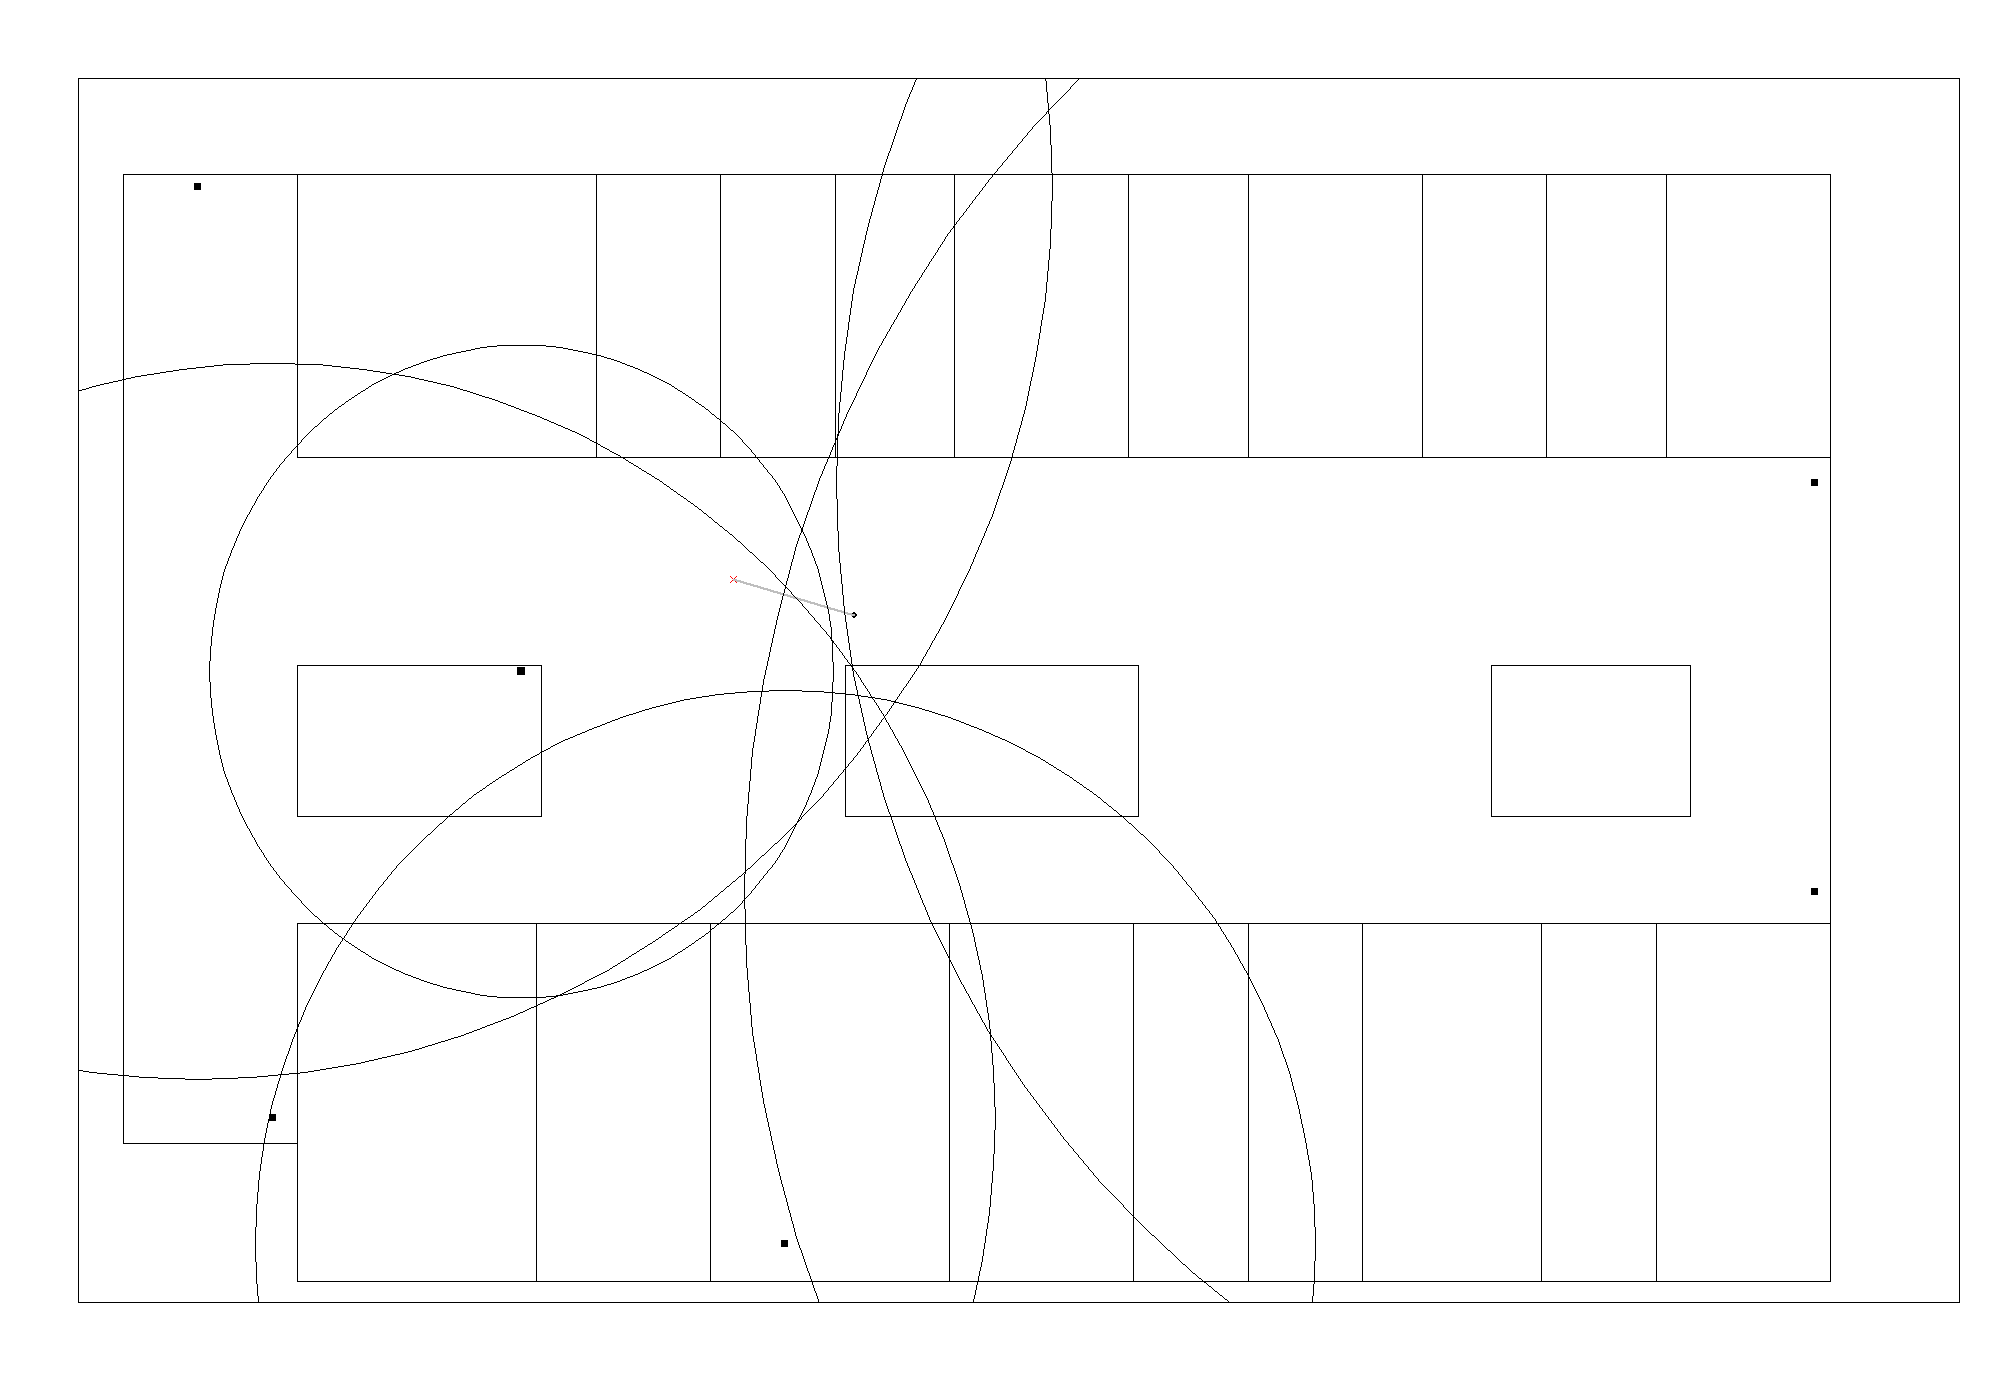
\includegraphics[width=\columnwidth]{img/circles_real4.png}}
  \caption{Single example of Trilateration Technique given predicted distances}
  \label{fig: Distance Comparison}
\end{figure}

The following chart shows the predicted and actual locations for the online validation dataset. The average error in the distance for this method is 4.96 meters.

\begin{figure}[htbp]
  \centerline{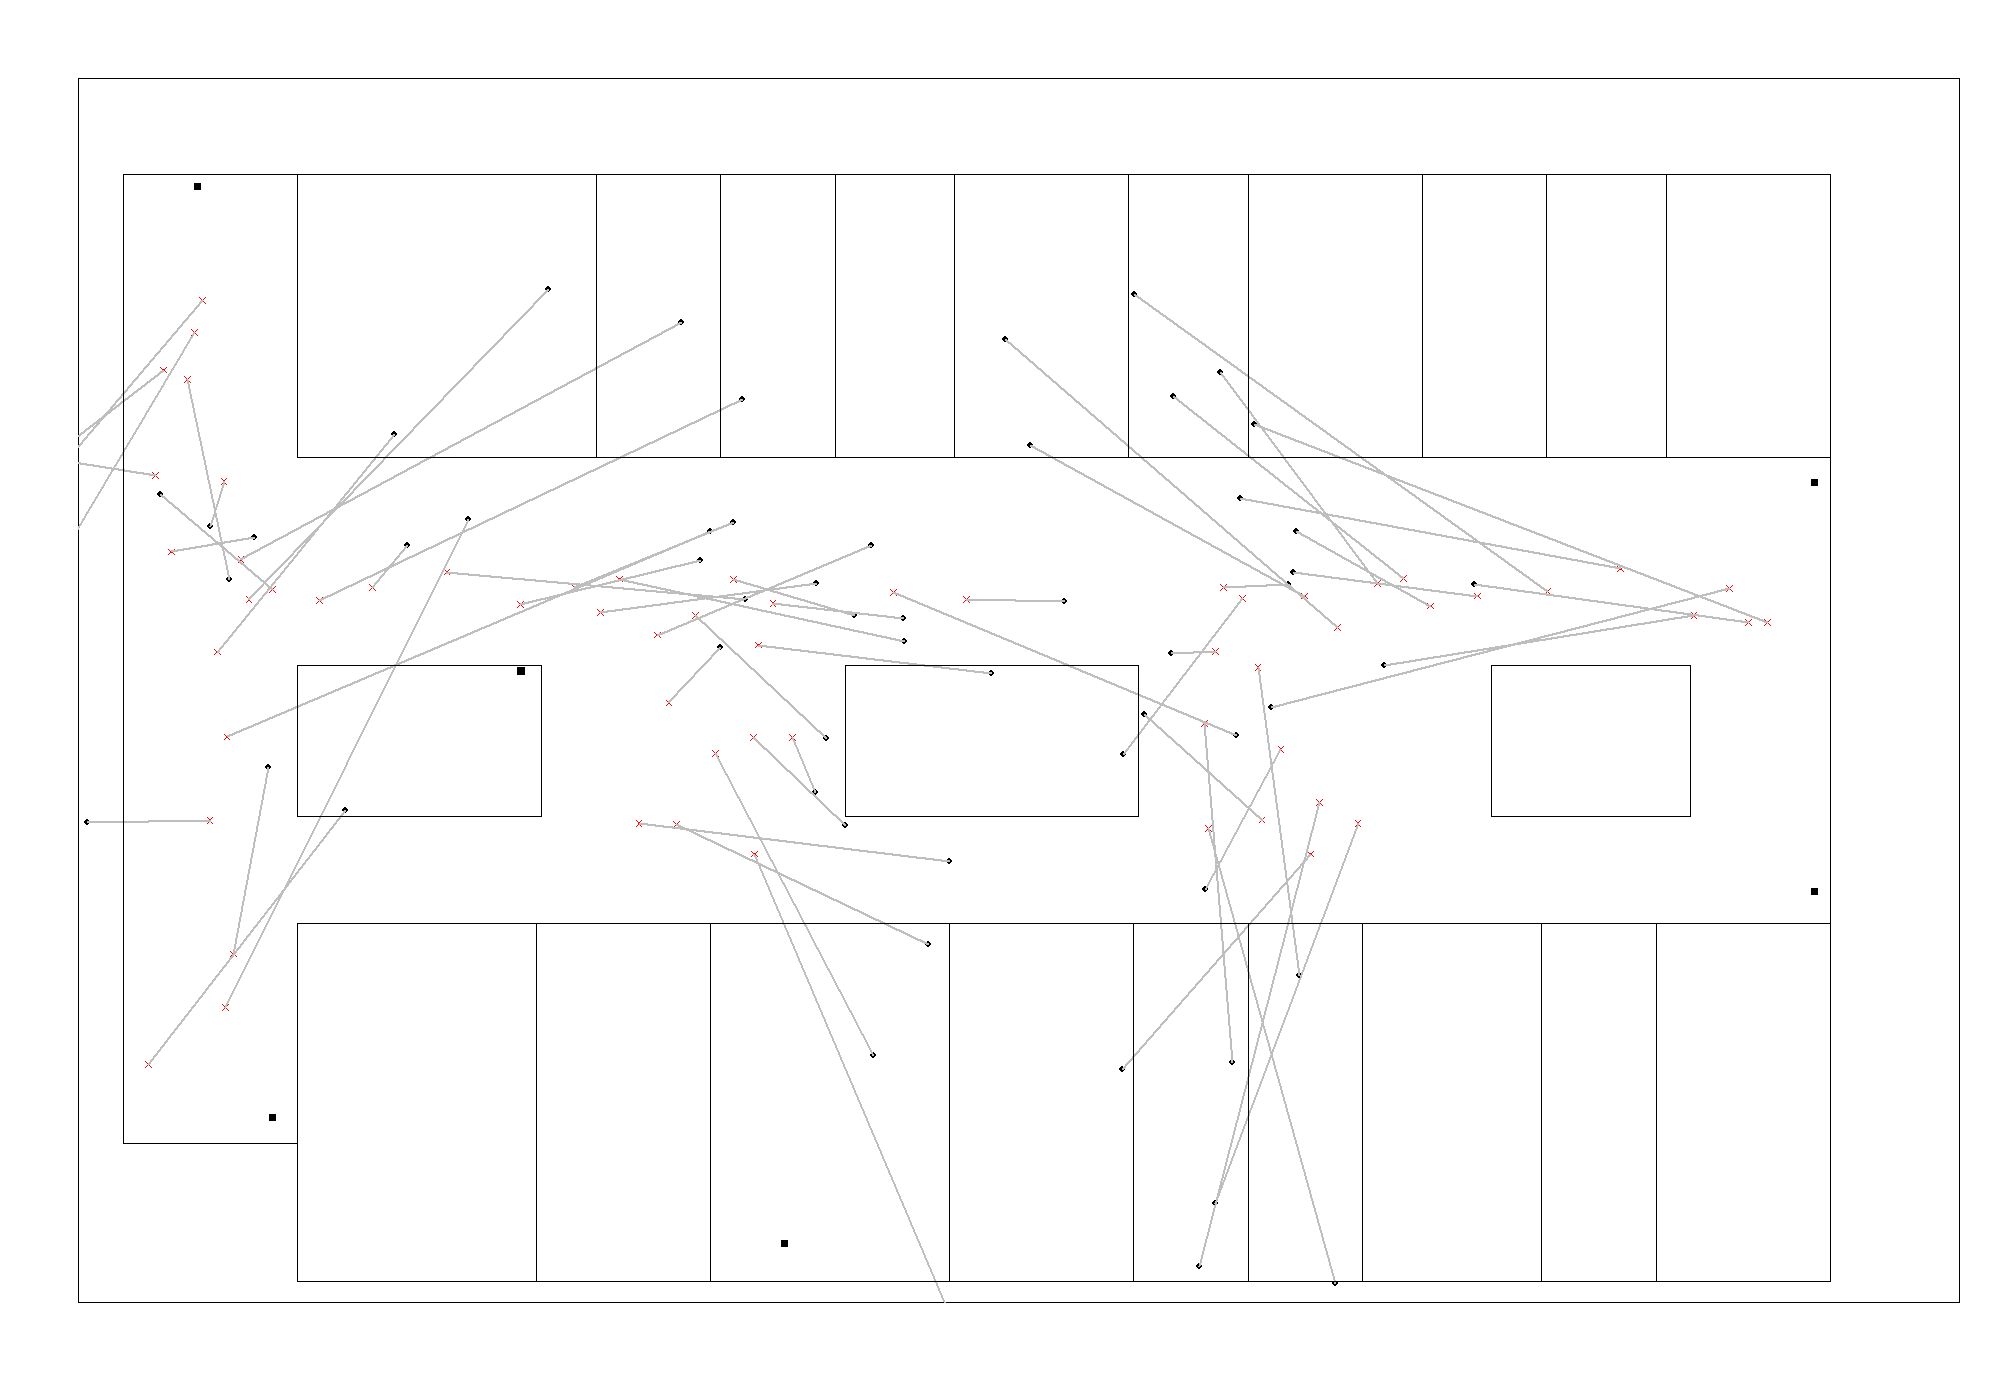
\includegraphics[width=\columnwidth]{img/Multilateration_Error.png}}
  \caption{Floor plan of estimated device locations for Trilateration Techinque}
  \label{fig: Trilateration Floor Plan}
\end{figure}


\subsection{K-Nearest Neighbor}
The second method we adopted is using the K-nearest Neighbors (KNN) Classification algorithm in order to predict the locations of our devices from the online dataset. The procedure of this method is as follows: we first have our entire dataset consisting of offline and online data, we then transform the offline data as our training dataset and online data as our testing dataset. Since the testing dataset has records of RSSI values from various locations, we take these RSSI values compared with the close neighbors (in terms of RSSI) from our training dataset. By close, we mean finding similar RSSI values from the training dataset under the assumption that the predicted location has the same MAC address and orientation as the actual location of the testing dataset. We define $k$ as the number of neighbors in the training set, then the corresponding positions of our neighbors will be considered as the predicted positions in the test dataset. The neighbors are defined to be 
$$
  \text{min}\left(\sqrt{(RSSI_{train}-RSSI_{test})^2}\right), k=1.
$$ 
If $k>1$, then we choose the least $k$ numbers of RSSI values as our neighbors.


Now that we have the basic procedures as to how to find the predicted positions, this brings up a new question as to how many neighbors should we select? The choice of $k$ is very sensitive, choosing a small amount of $k$ leads to underfitting of our model to the training data, and choosing a large amount of $k$ leads to overfitting. Ideally, we want to choose the value of $k$ that is independent from our test data, the method of $k$-fold Cross-Validation (CV) can help us do this.

The idea behind $k$-fold CV is quite simple: we first divide our training data into numerous non-overlapping subsets of equal size. Then for each subset, we build models with the data that are not in that subset and we assess the predictive ability of the model using the subset that was left out. We repeat this model fitting and assessment for each fold and aggregate the prediction errors across the folds. The prediction errors are denoted as 
$$
  \text{SSE}(XY_{act}-XY_{est}),
$$ 
where SSE stands for Sum of Squares Error or Sum of Squares Residuals, representing the difference between the actual position and the estimated position of devices (see Fig~\ref{fig: K-Fold CV}).
\begin{figure}[htbp]
  \centerline{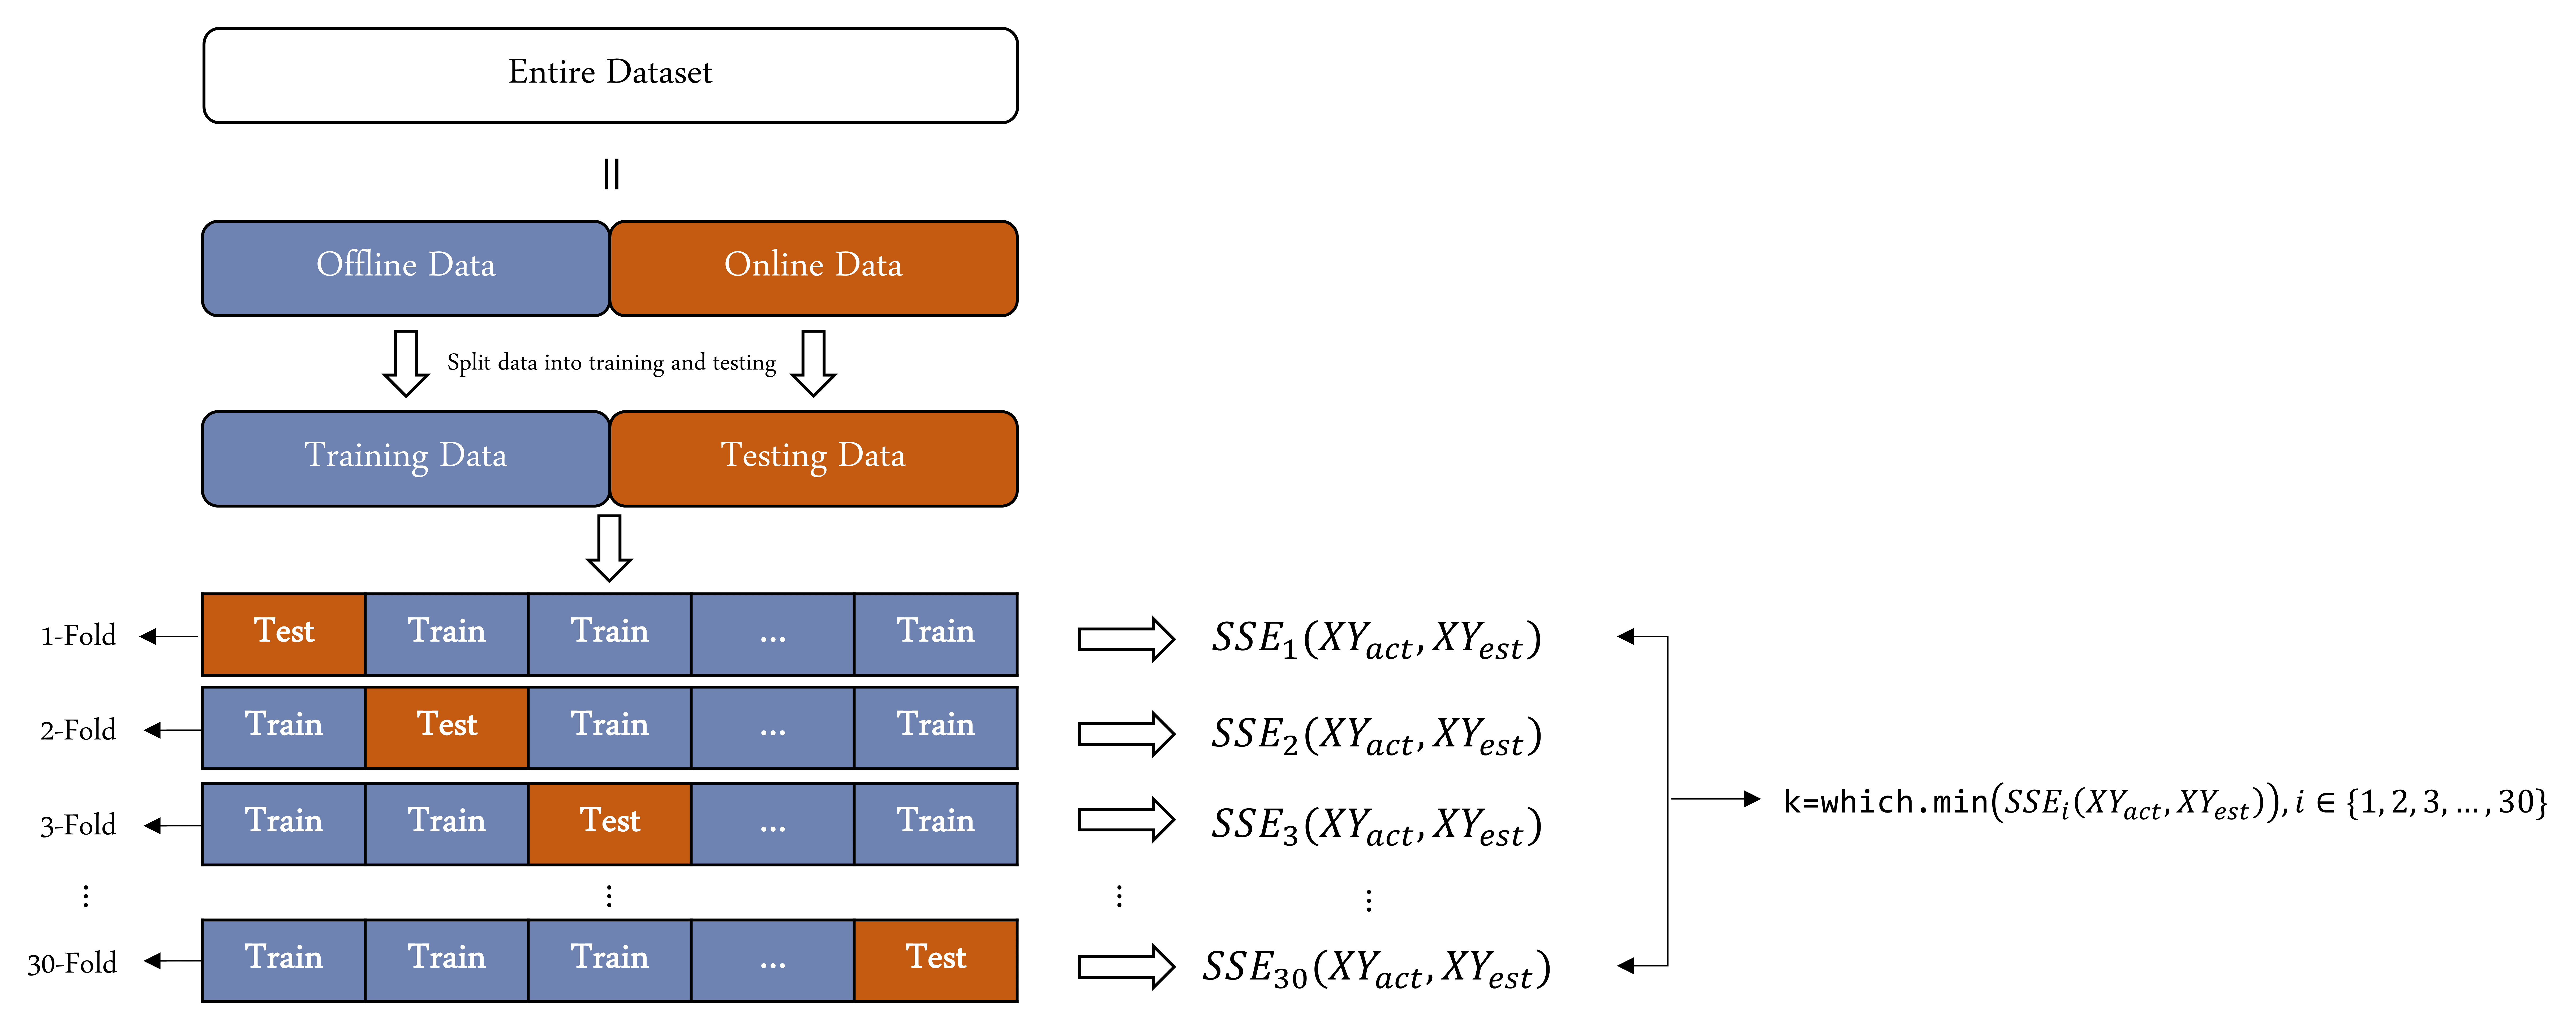
\includegraphics[width=\columnwidth]{img/K-Fold CV.png}}
  \caption{Schematic diagram of K-fold Cross-Validation}
  \label{fig: K-Fold CV}
\end{figure}

\begin{figure}[htbp]
  \centerline{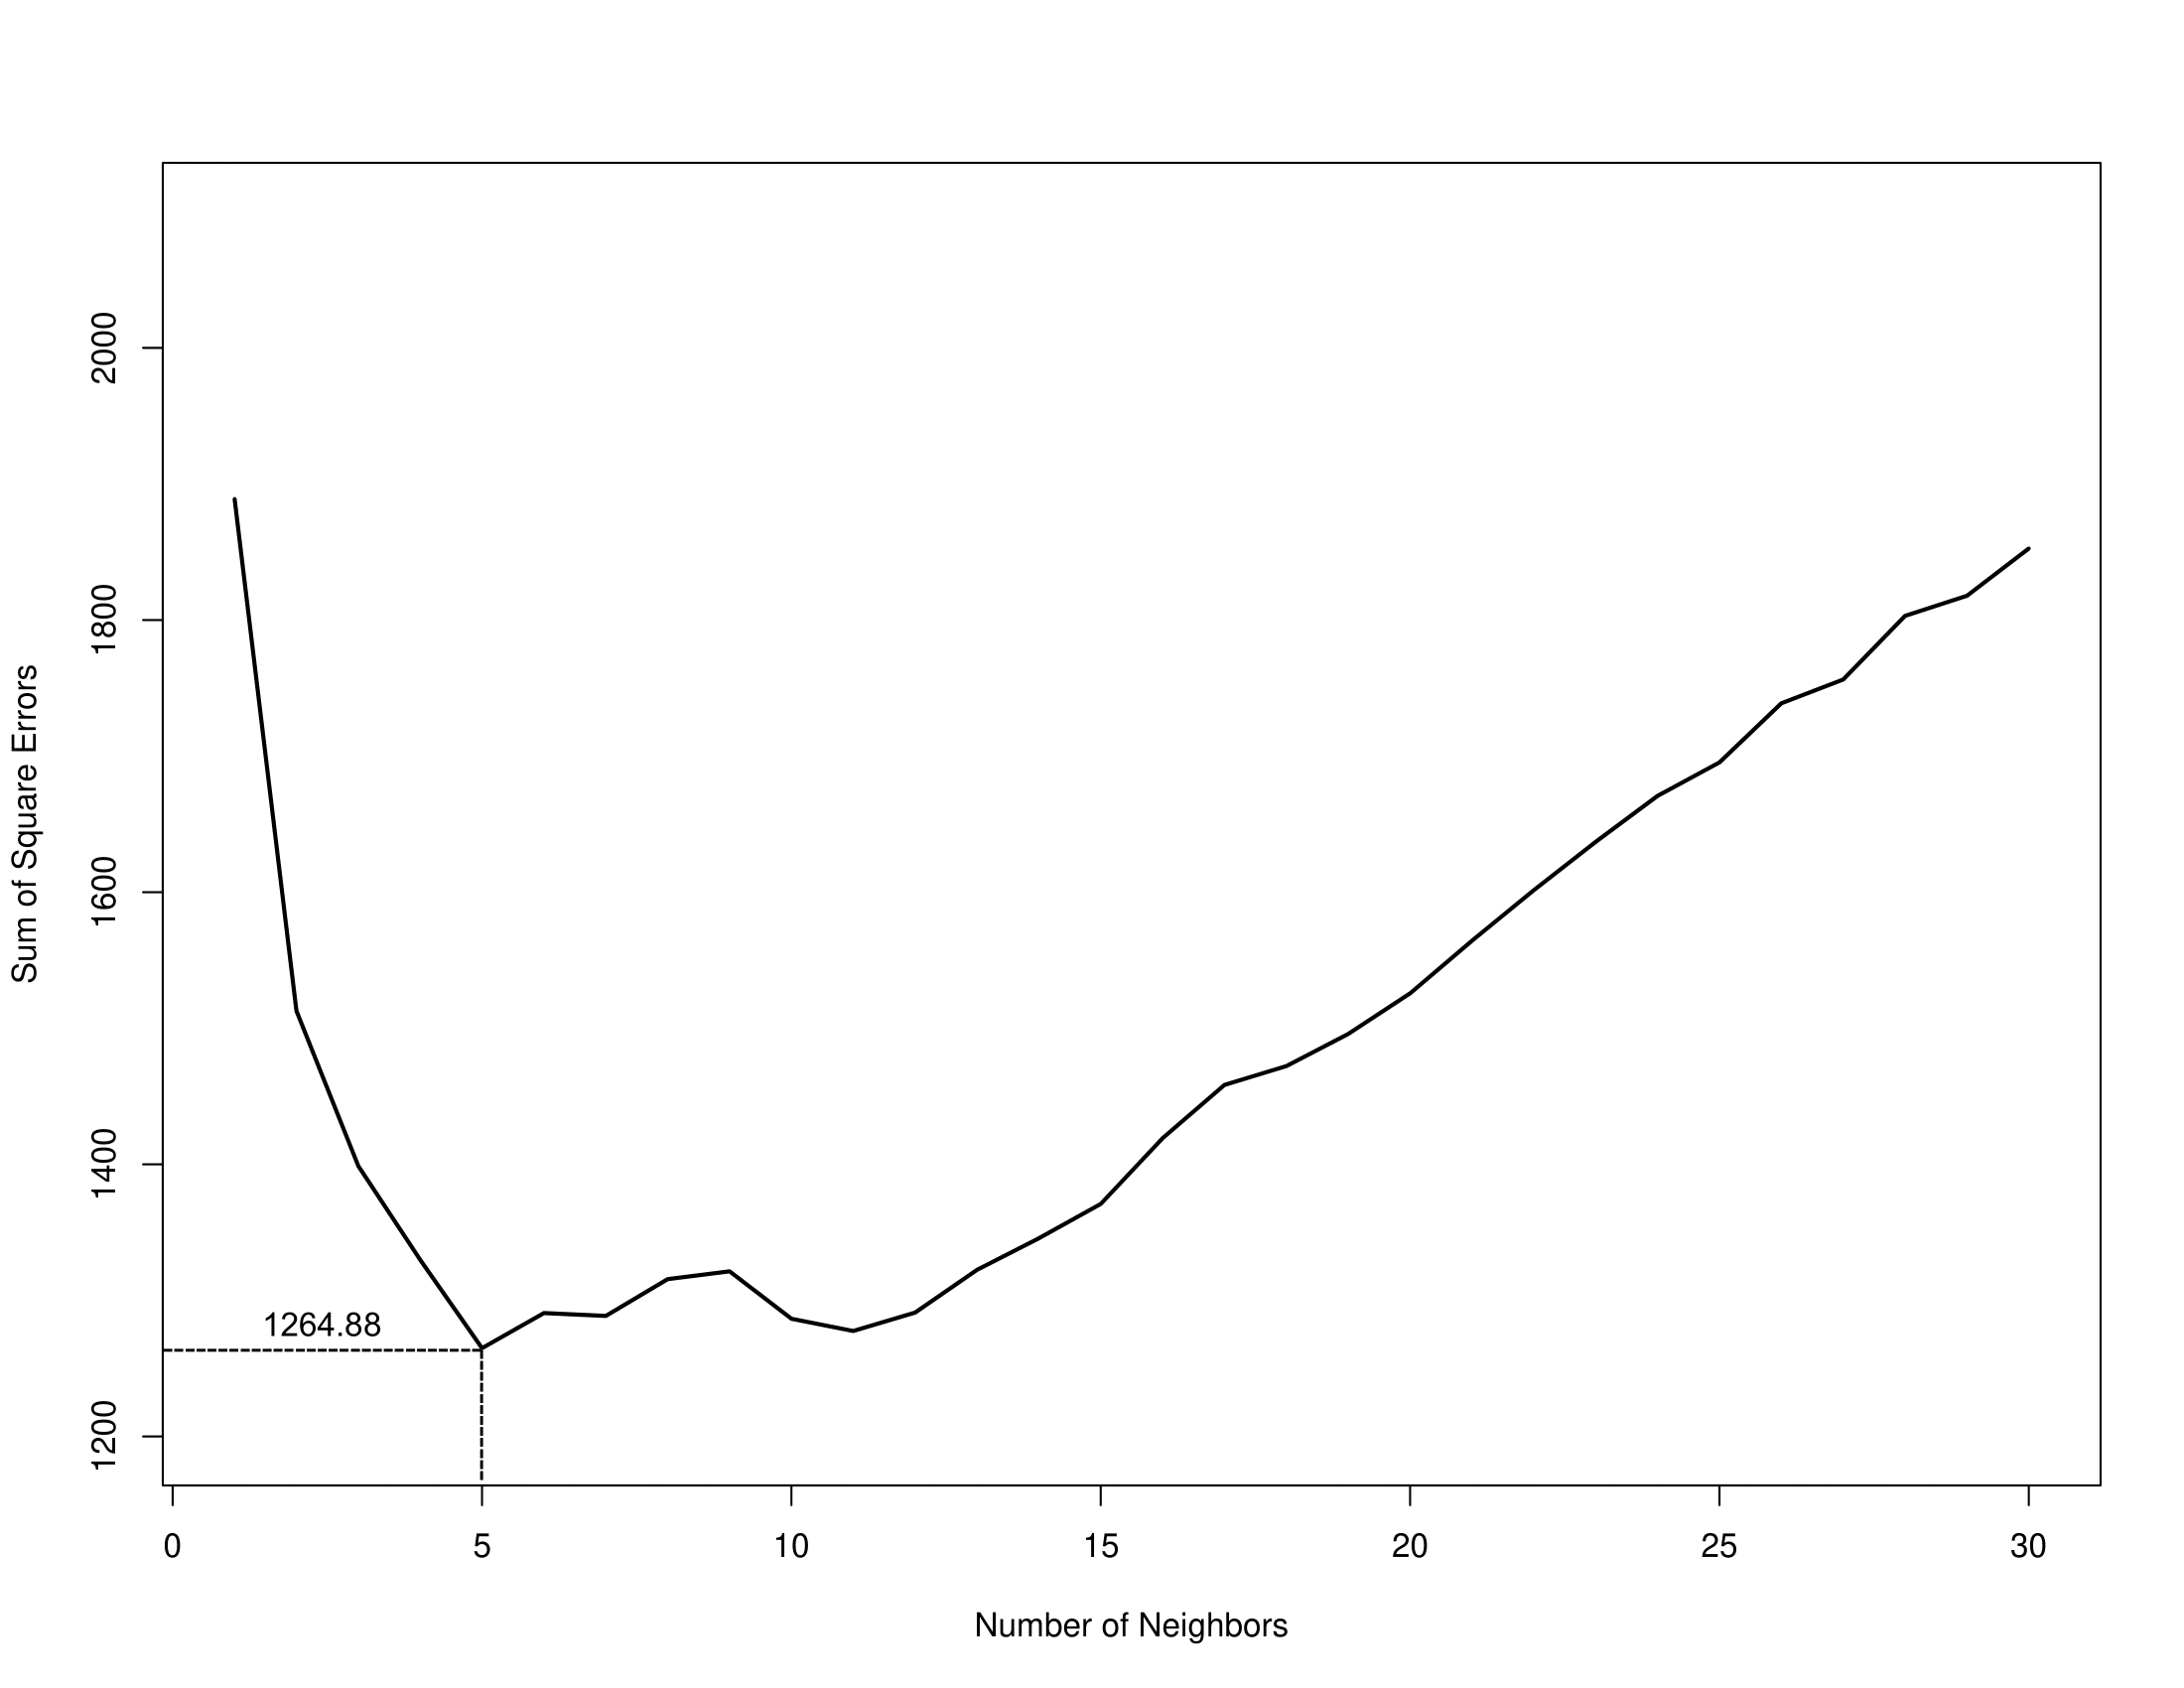
\includegraphics[width=\columnwidth]{img/Plot-k-fold_CV-1.png}}
  \caption{Schematic diagram of K-fold Cross-Validation}
  \label{fig: Choice of K}
\end{figure}
As the above figure shows, the SSE is lowest when $k=5$, suggesting us that 5 neighbors will give us the least error between estimated positions and actual positions.

\begin{figure}[htbp]
  \centerline{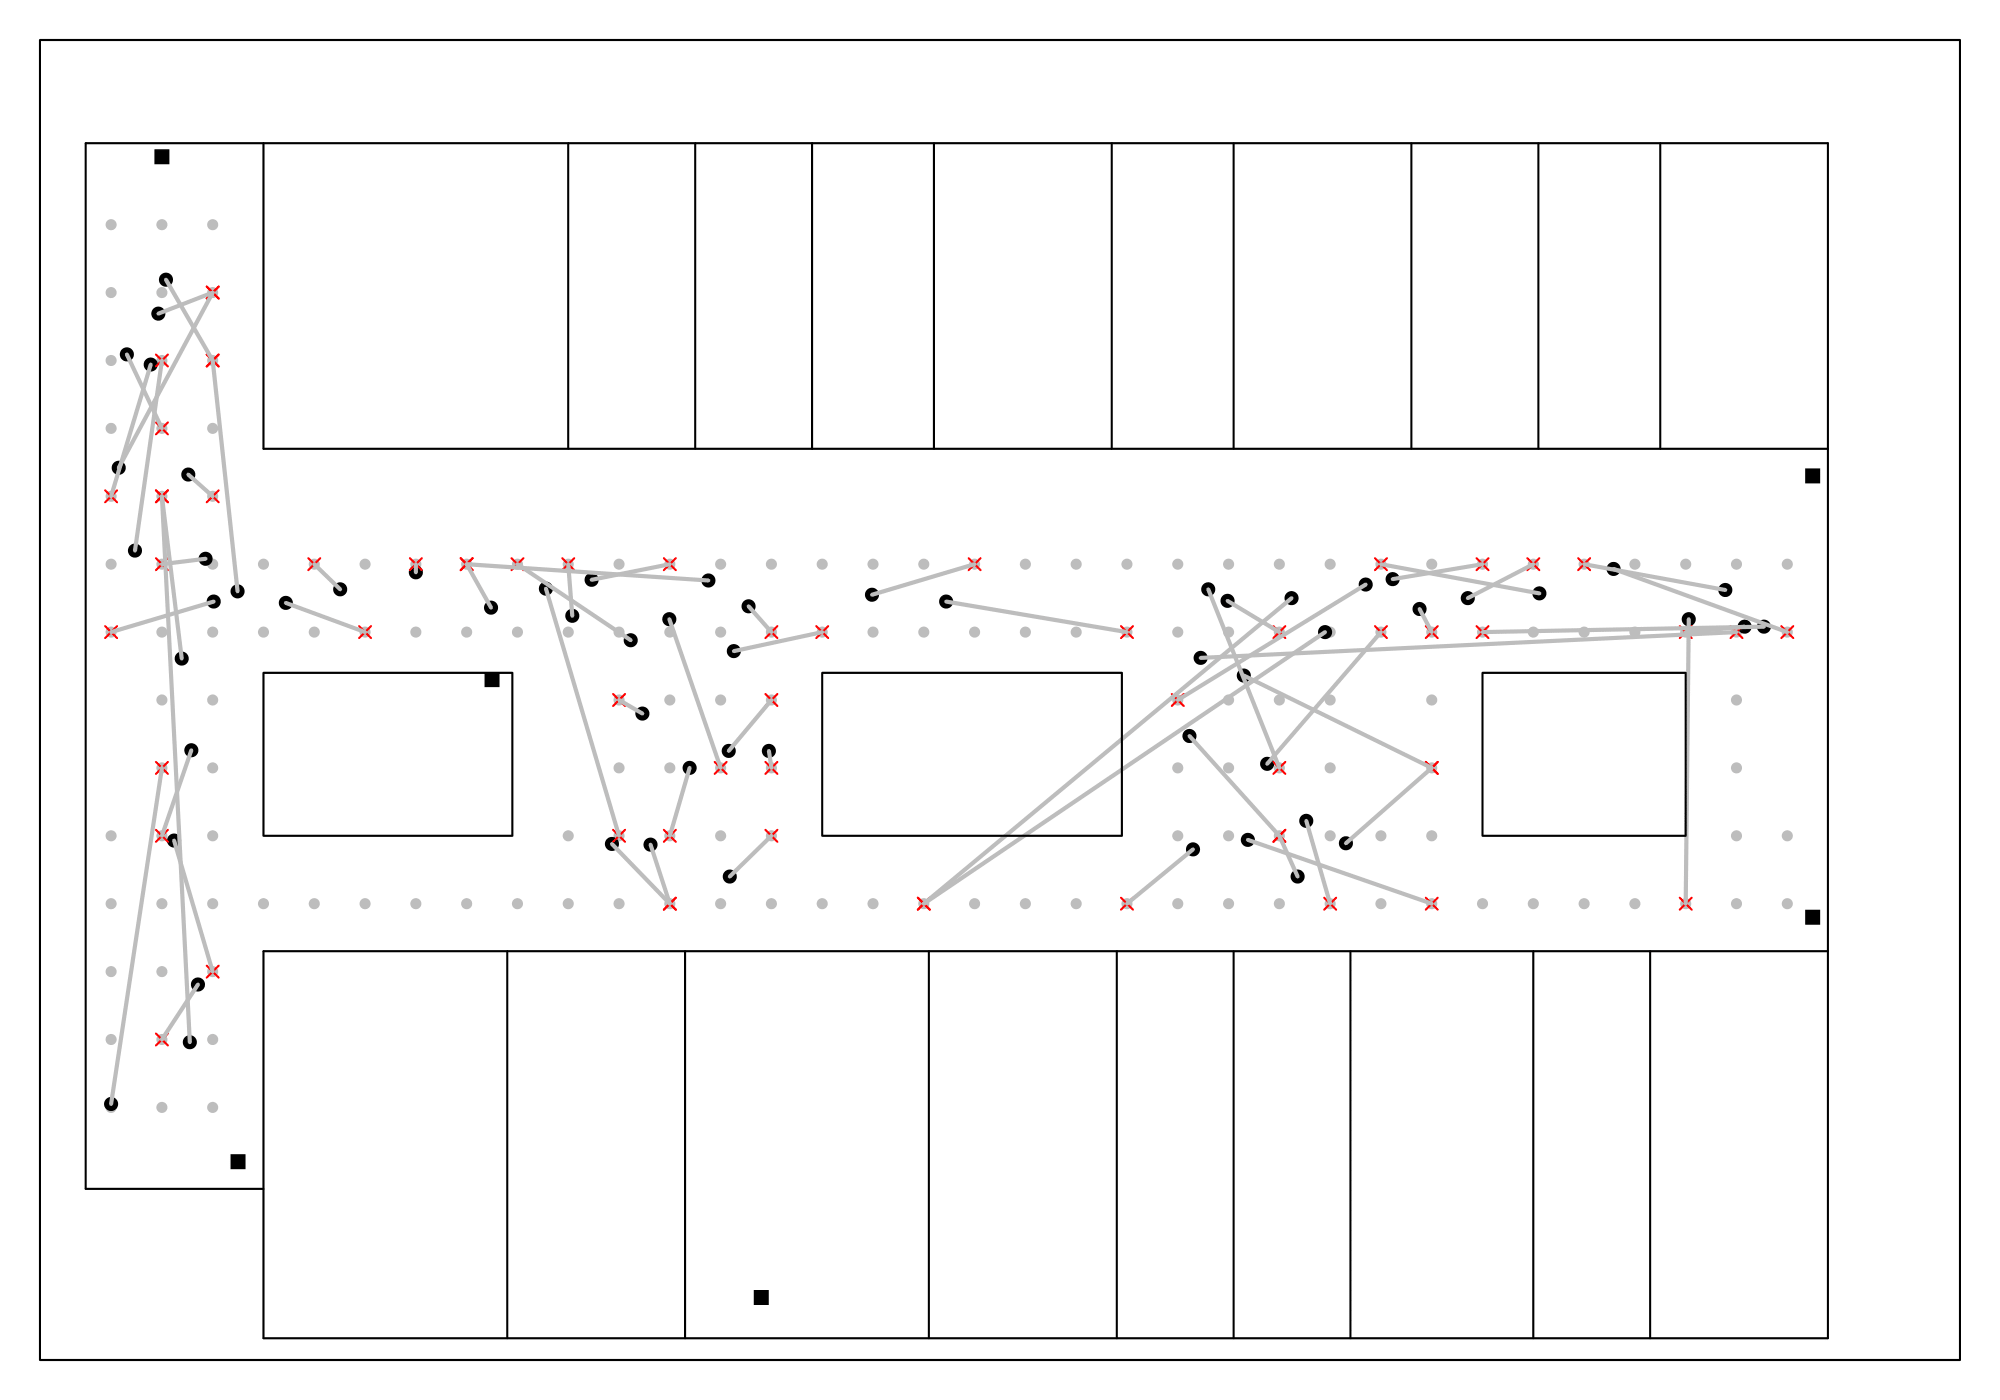
\includegraphics[width=\columnwidth]{img/Plot-K1FloorPlan-1.png}}
  \caption{Floor plan of estimated device locations when $k=1$}
  \label{fig: K1}
\end{figure}

\begin{figure}[htbp]
  \centerline{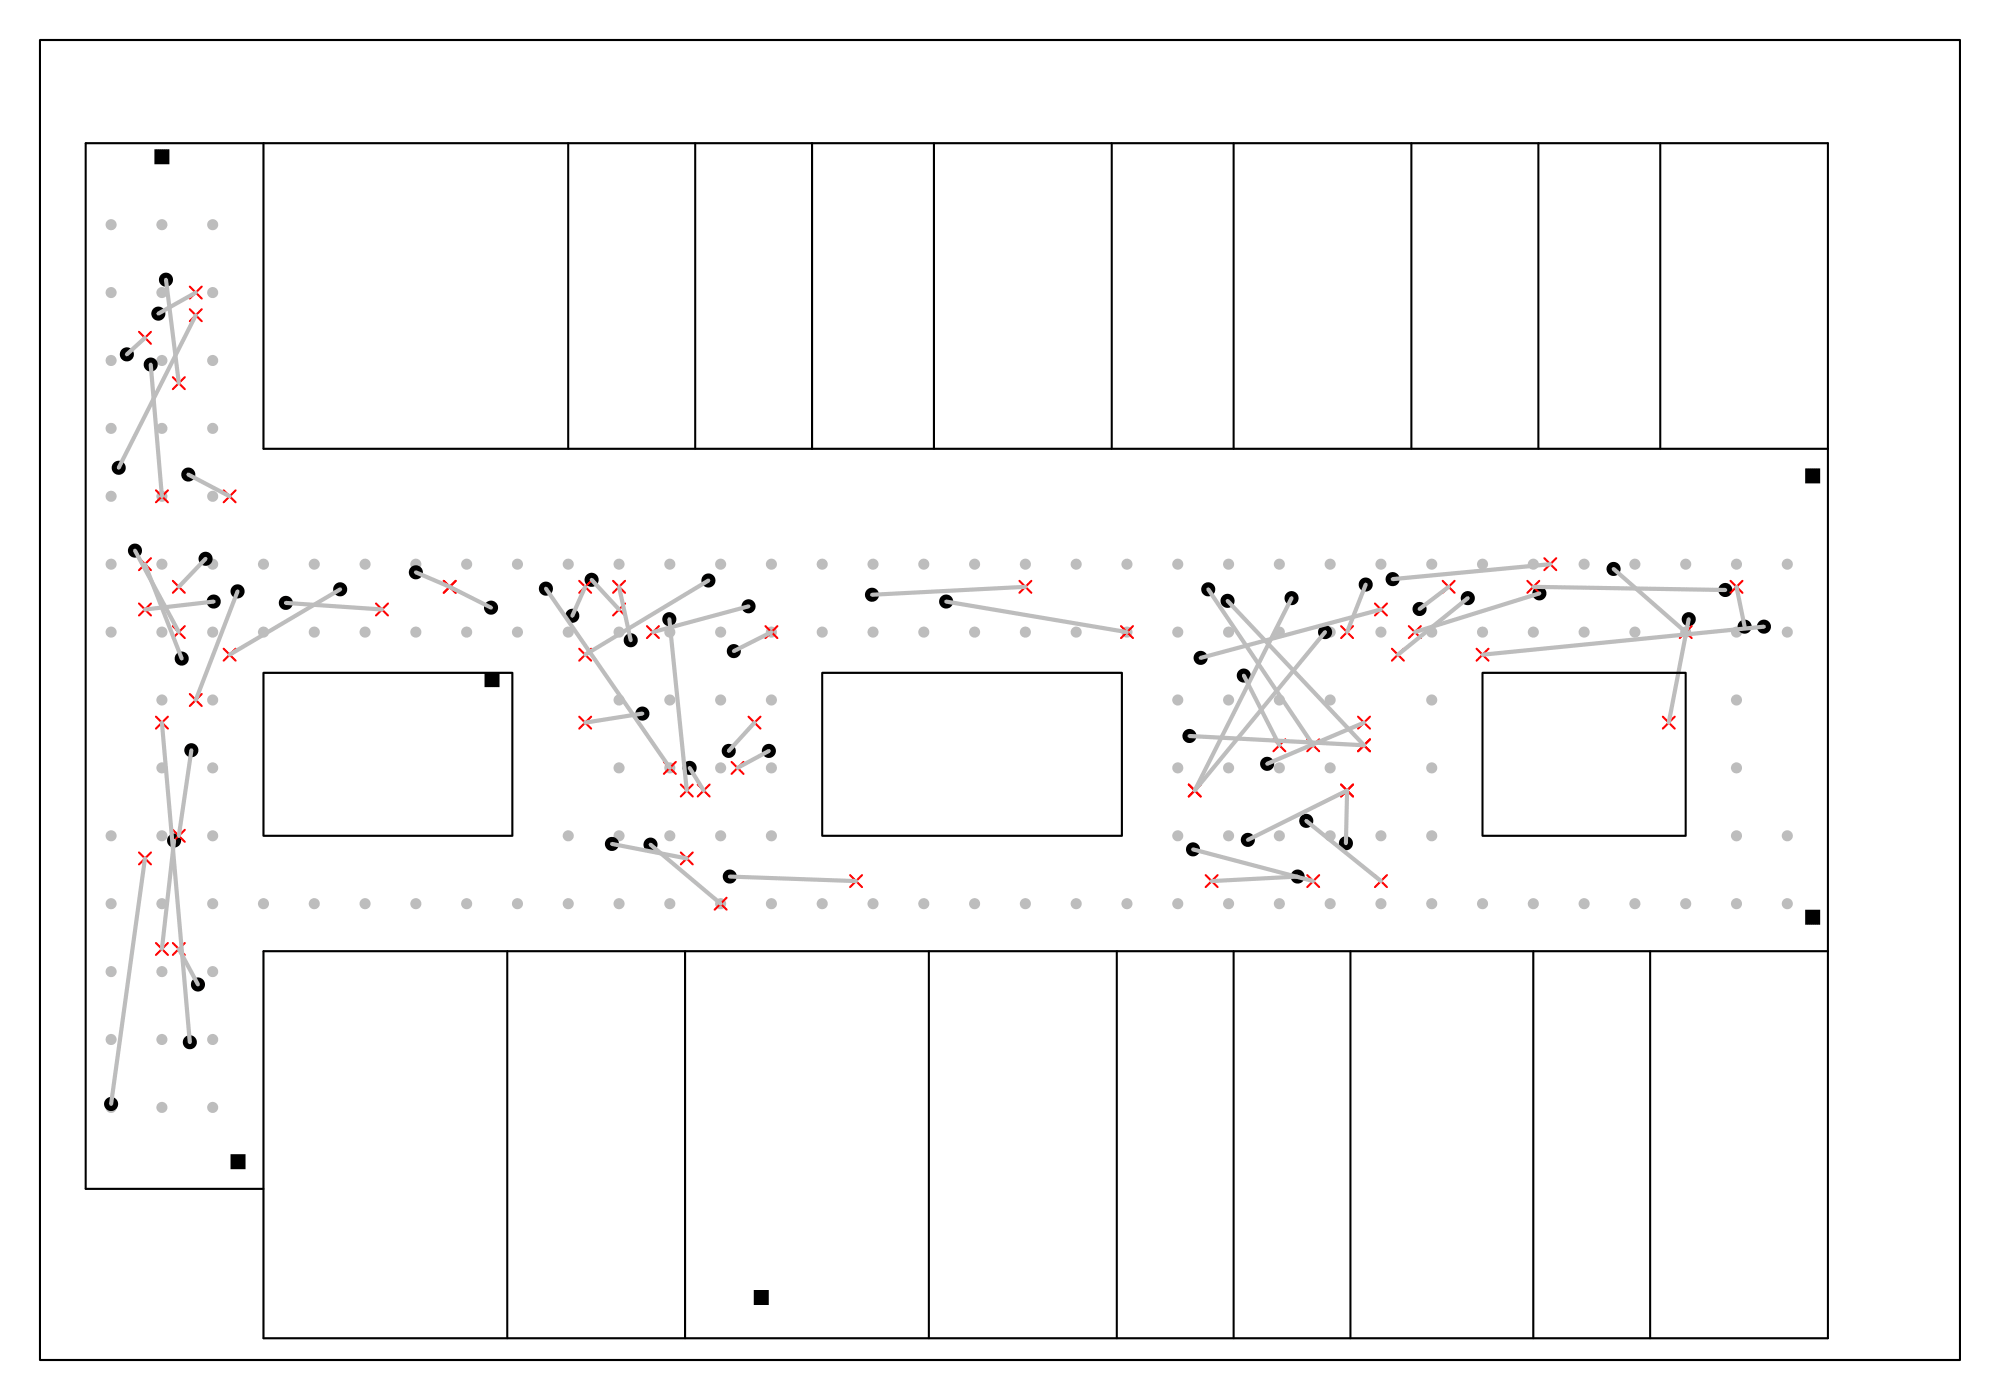
\includegraphics[width=\columnwidth]{img/Plot-K3FloorPlan-1.png}}
  \caption{Floor plan of estimated device locations when $k=3$}
  \label{fig: K3}
\end{figure}

\begin{figure}[htbp]
  \centerline{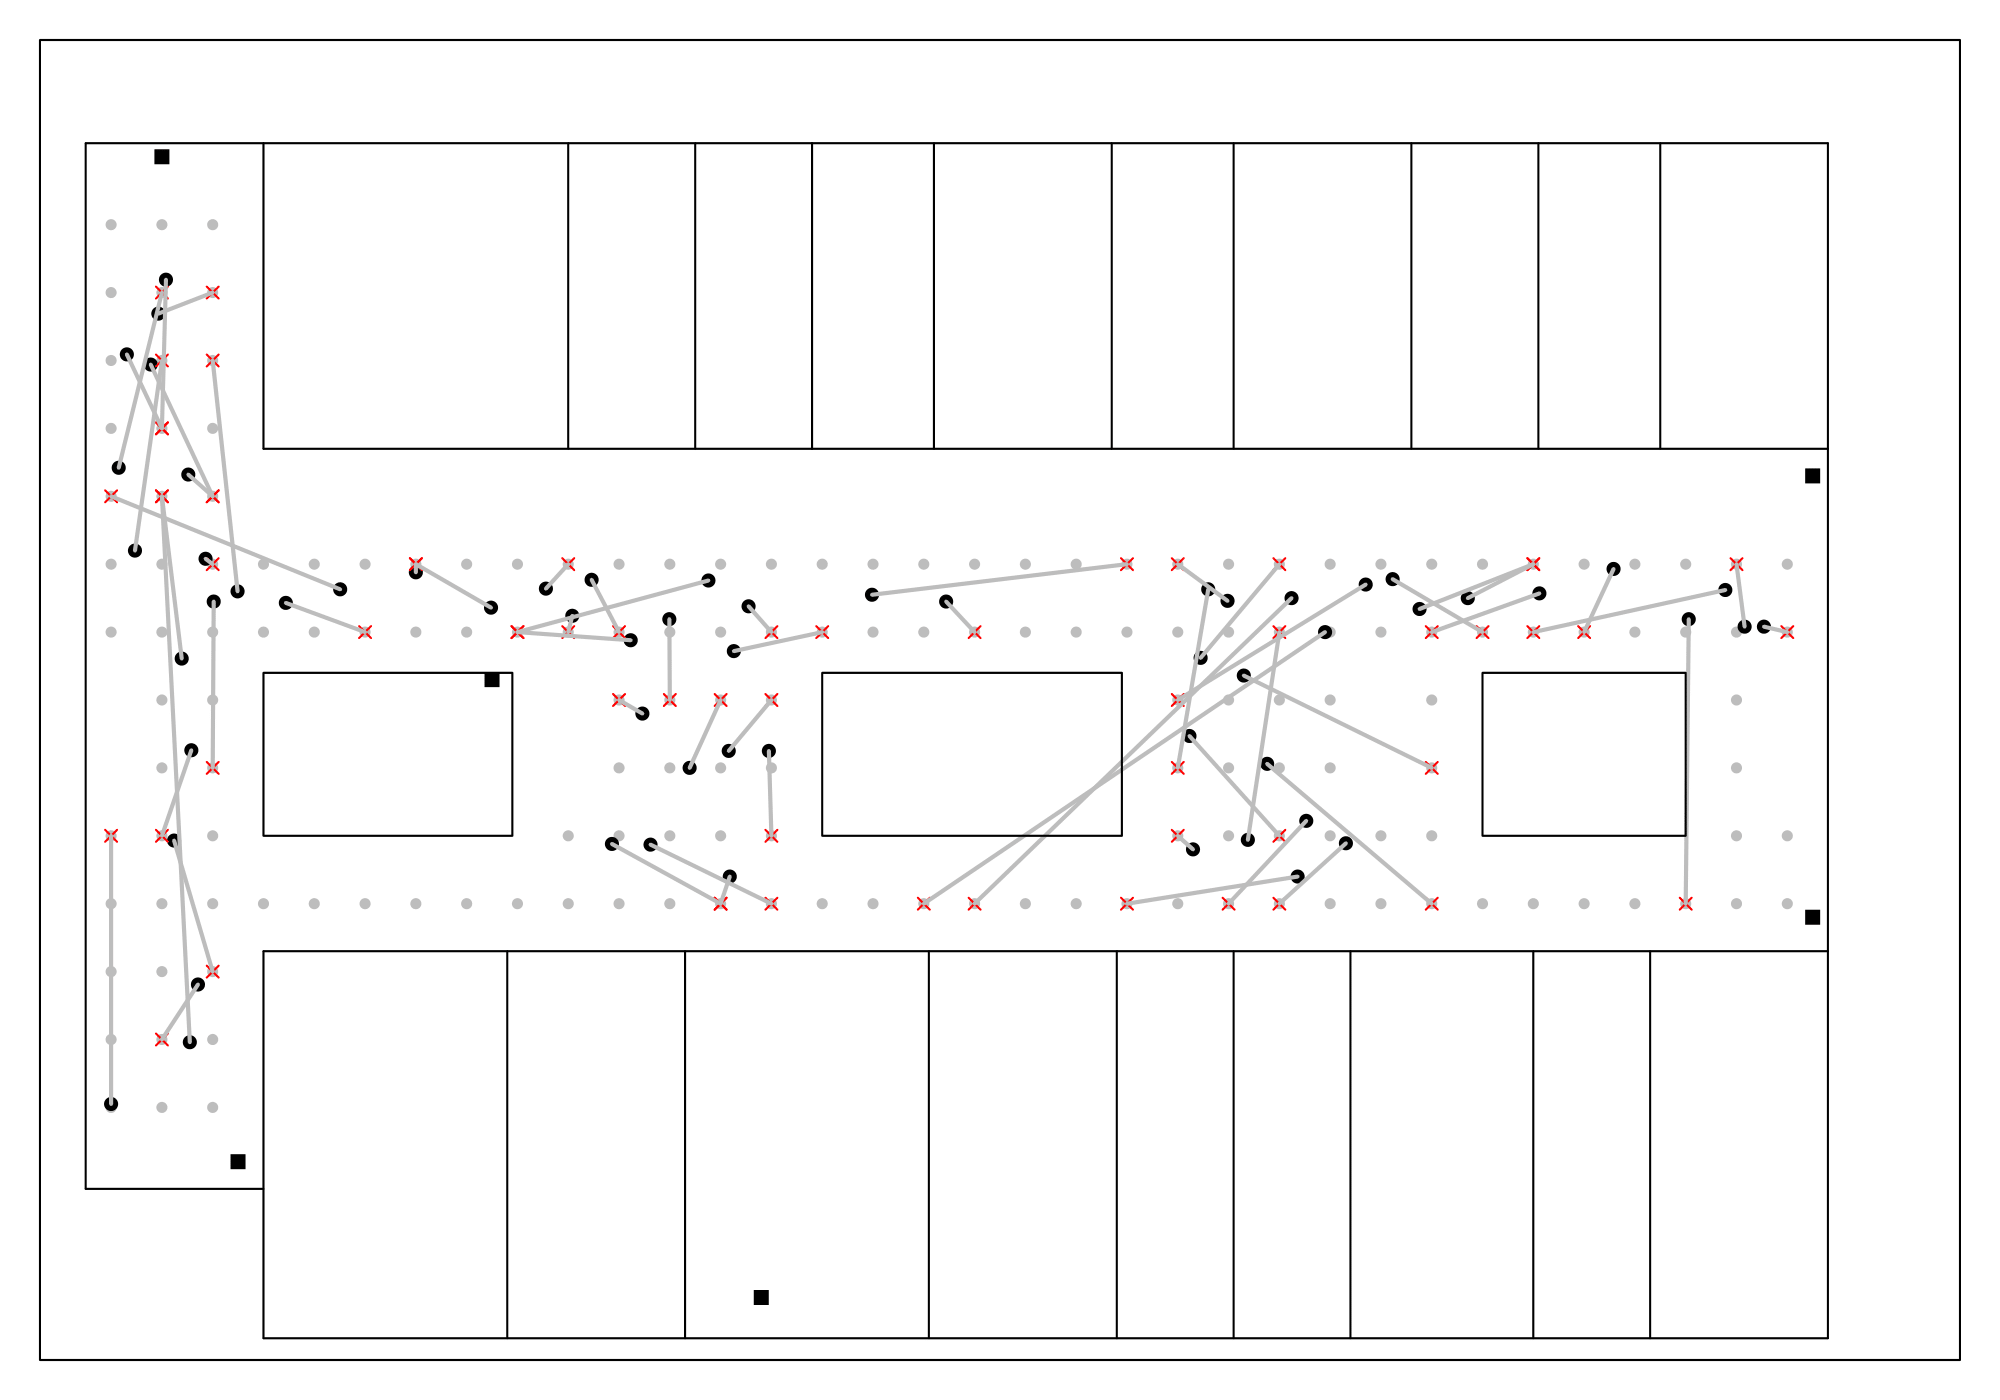
\includegraphics[width=\columnwidth]{img/Plot-K5FloorPlan-1.png}}
  \caption{Floor plan of estimated device locations when $k=5$}
  \label{fig: K5}
\end{figure}

The below 3 figures are the floor plan views of our dataset, the grids are the actual classrooms, the gray points are the training dataset, the black points are the testing dataset, the black squares being the access points, and the black lines indicates the error between the actual and estimated positions.

We can see that $k=3$ shows a much smaller error in distance than $k=1$. While the plot for $k=5$ is similar to the plot for $k=1$, the average and median error in distance is actually smaller in $k=5$.

\begin{table}[htbp]
  \begin{tabular}{|l|c|c|}
  \hline
  # of $k$   & Average Error Distance & Median Error Distance \\ \hline
  $k=1$        & 2.517842 m             & 1.902775 m            \\ \hline
  $k=3$        & 1.931918 m             & 1.662997 m            \\ \hline
  $k=5$        & 1.769582 m             & 1.412887 m            \\ \hline
  \end{tabular}
\end{table}

%------------------------------------------------------------------------------------------------------------------------------------
% Evaluation
%------------------------------------------------------------------------------------------------------------------------------------
\section{Evaluation}
\begin{figure}[htbp]
  \centering
  \subfigure[Trilateration Prediction]{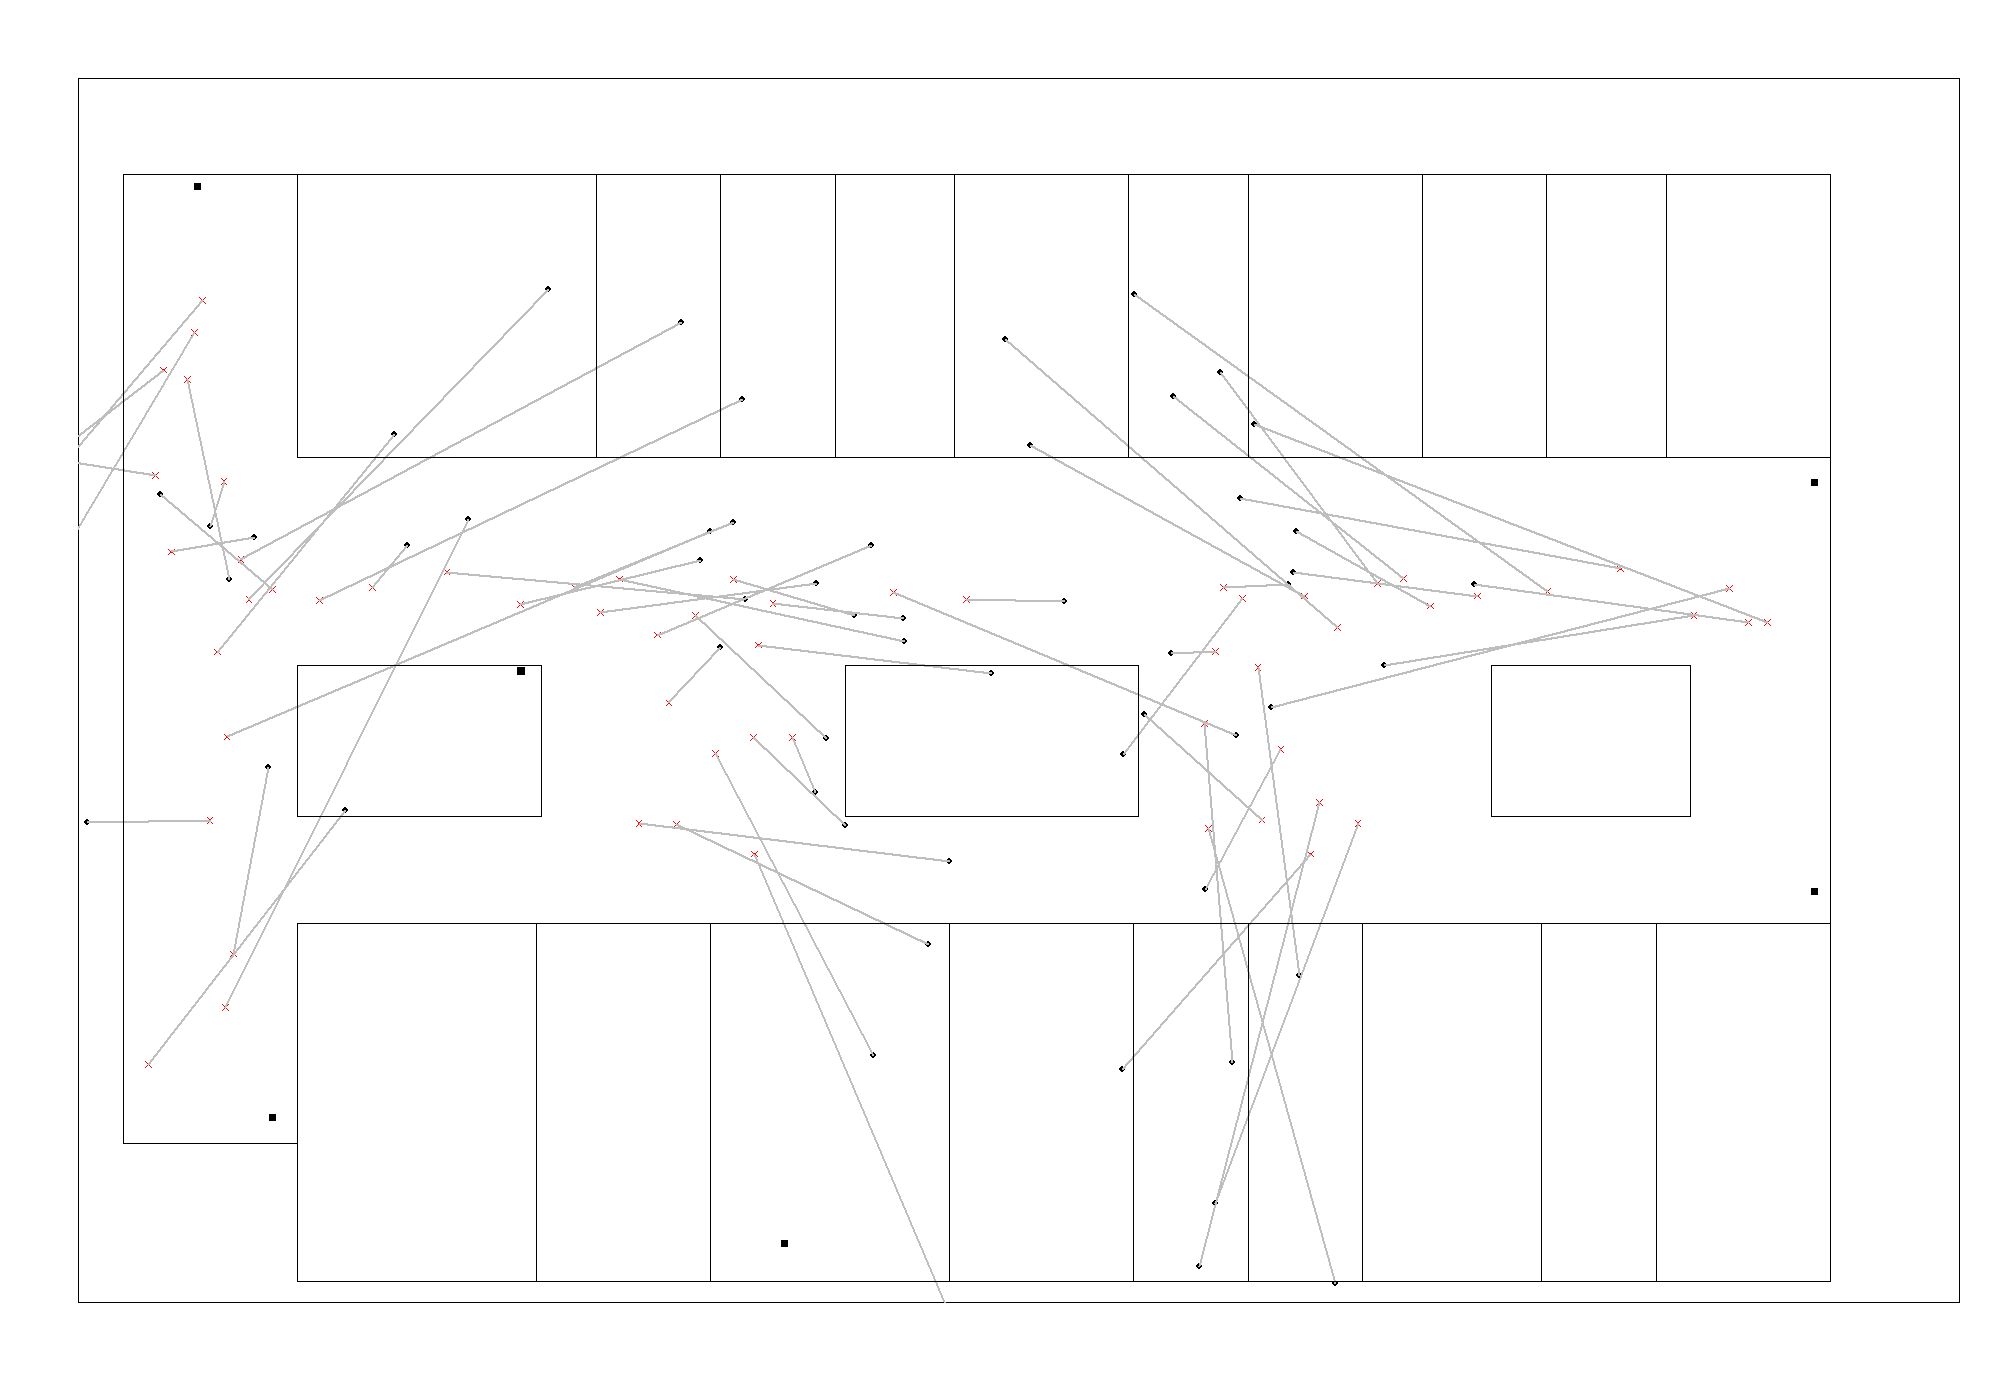
\includegraphics[width=0.24\textwidth]{img/Multilateration_Error.png}}
  \subfigure[KNN Prediction]{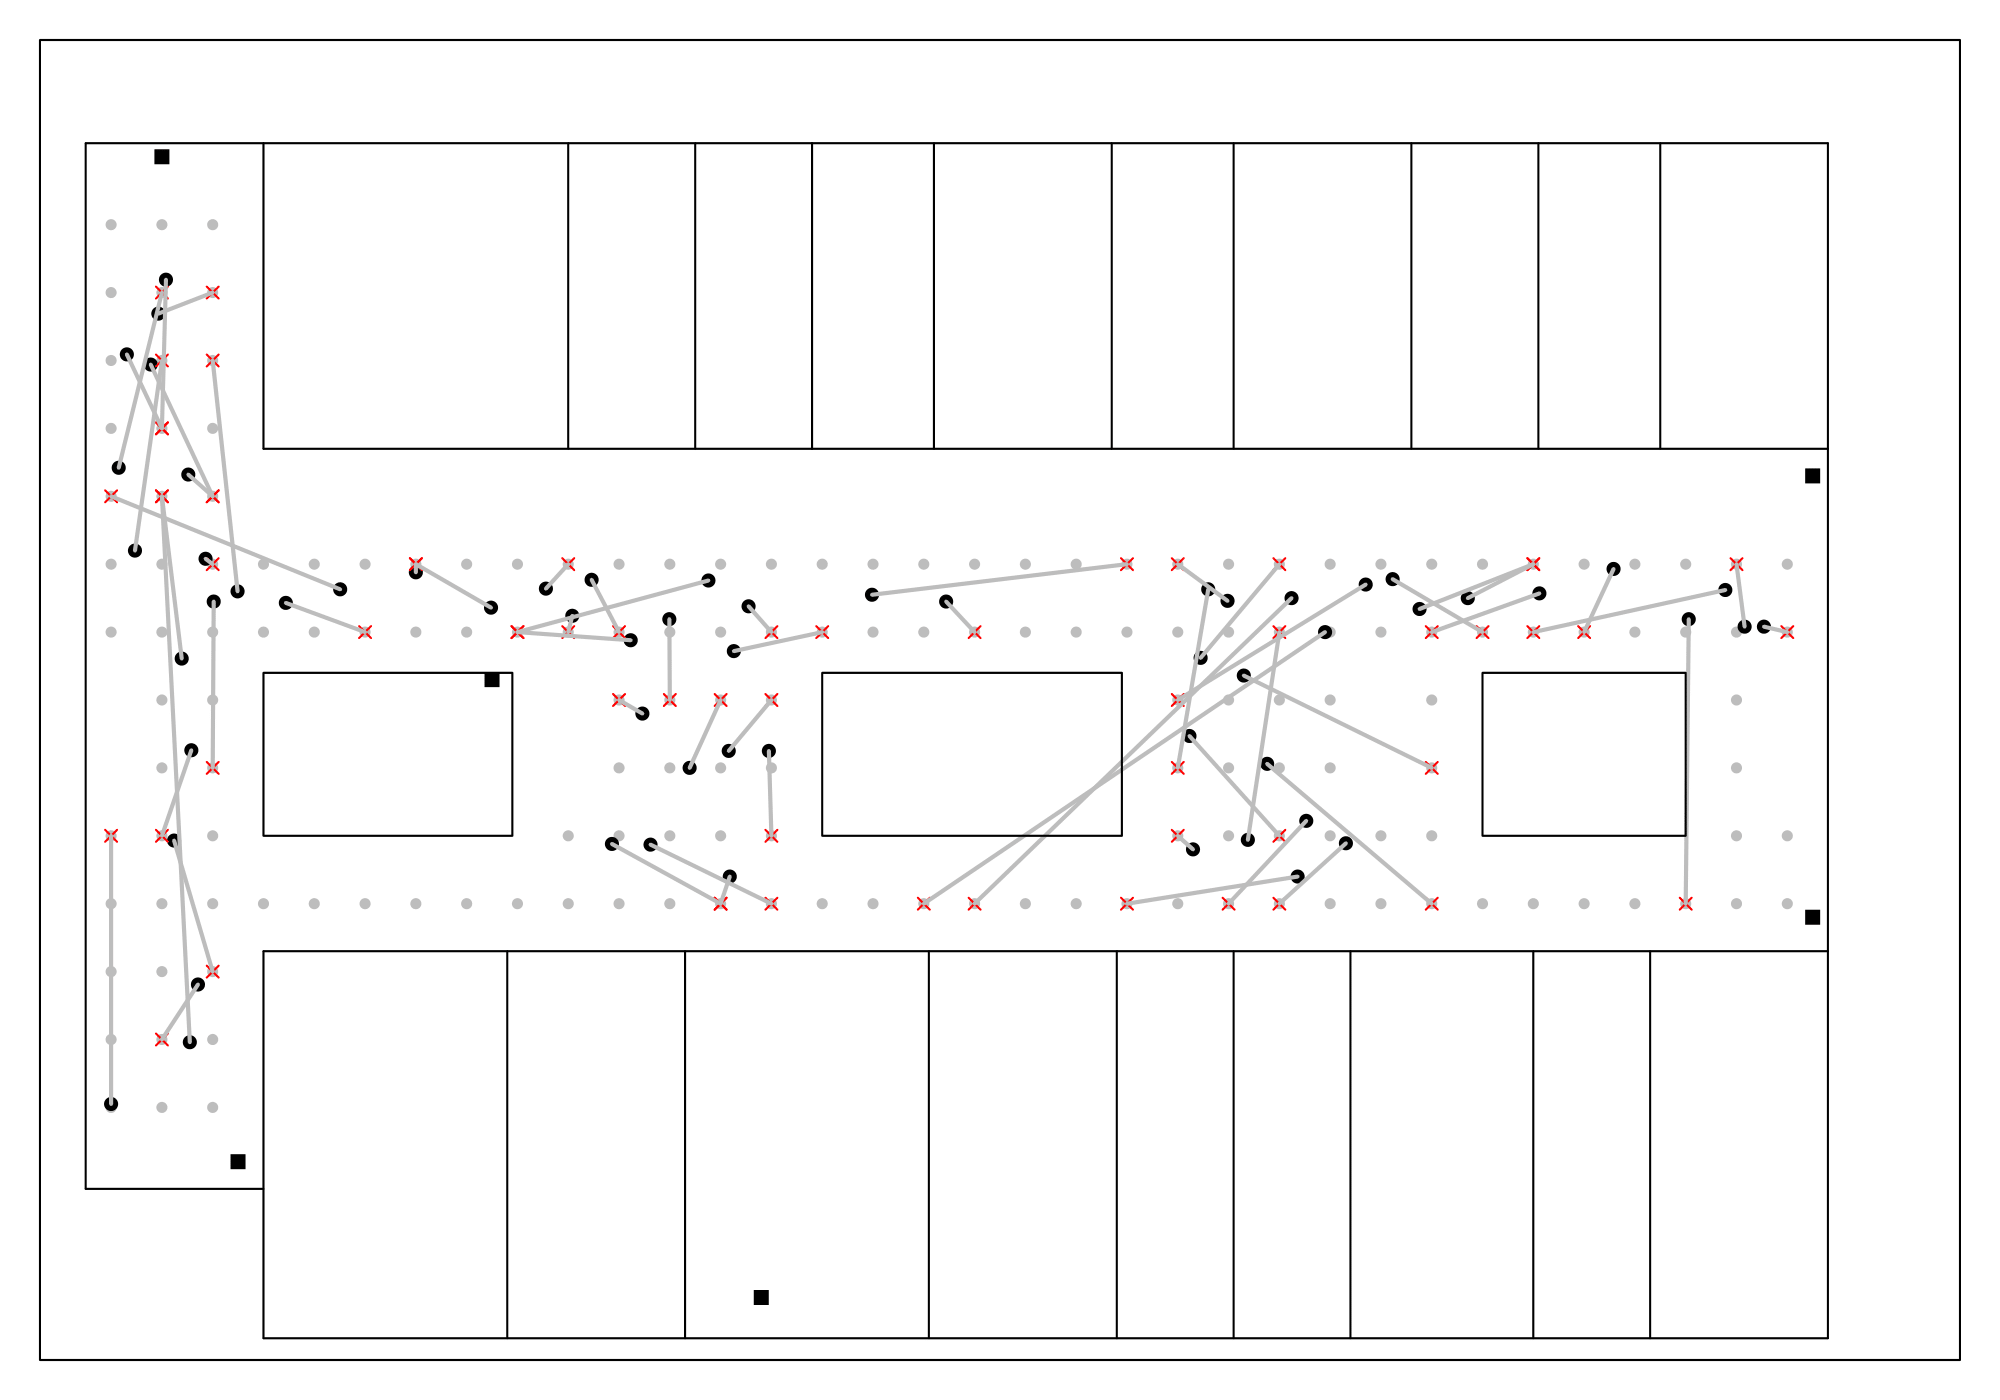
\includegraphics[width=0.24\textwidth]{img/Plot-K5FloorPlan-1.png}}
  \caption{Error of distance using 2 methods}
  \label{fig: Comparison}
\end{figure}

\begin{table}[htbp]
  \begin{tabular}{|l|c|c|}
  \hline
  Method        & Average Error Distance & Median Error Distance \\ \hline
  Trilateration & 4.832989 m             & 4.955922 m            \\ \hline
  KNN           & 2.517842 m             & 1.902775 m            \\ \hline
  \end{tabular}
\end{table}

Referring to the above table, we can see that the mean and median error distance using the KNN algorithm are much lower than those using Trilateration Technique.

%------------------------------------------------------------------------------------------------------------------------------------
% Conclusion
%------------------------------------------------------------------------------------------------------------------------------------
\section{Conclusion}
Originally, we were tasked with providing consulting services regarding developing Wi-Fi localization. Our client wanted the ability to identify the physical location of devices that were connected to their network. Therefore, our goal was to create a model or methodology that is capable of taking a set of received signal strengths (RSSI) values from relevant broadcasting wireless access points and estimating the location of that device. Additionally, our client wanted the model to include the accuracy of the prediction to establish a degree of accuracy/error. Our team thoroughly examined the data provided by the client, researched multiple possible models that could be presented to the client to establish a greater contextual understanding, and were able to meet all requirements set for our team. While the multilateration didn't completely deliver in determining a position within an acceptable margin of error, there is still room for improvement to further fine tune the model where it could serve the role as being a contingency or for benchmarking purposes. Ultimately, the K-Nearest Neighbor algorithm is the model we recommend because of its higher degree of accuracy for predicting locations.


%------------------------------------------------------------------------------------------------------------------------------------
% Reference
%------------------------------------------------------------------------------------------------------------------------------------
\begin{thebibliography}{00}
\bibitem{b1} Babalola OP, Balyan V. WiFi fingerprinting indoor localization based on dynamic mode decomposition feature selection with hidden Markov model. Sensors. 2021 Oct 13;21(20):6778.
\newline
\bibitem{b2} Conesa J, Pérez-Navarro A, Sospedra JT, Montoliu R. Geographical and fingerprinting data to create systems for indoor positioning and indoor/outdoor navigation. Elsevier: Amsterdam, The Netherlands; 2018.
\newline
\bibitem{b3} Cramariuc A, Huttunen H, Lohan ES. Clustering benefits in mobile-centric WiFi positioning in multi-floor buildings. In2016 International Conference on Localization and GNSS (ICL-GNSS) 2016 Jun 28 (pp. 1-6). IEEE.
\newline
\bibitem{b4} Sansano-Sansano E, Montoliu Colás R, Belmonte-Fernández Ó, Torres-Sospedra J. Indoor Positioning and Fingerprinting: The R Package ipft.
\newline
\bibitem{b5} Liu F, Liu J, Yin Y, Wang W, Hu D, Chen P, Niu Q. Survey on WiFi‐based indoor positioning techniques. IET communications. 2020 Jun;14(9):1372-83.
\end{thebibliography}
\vspace{12pt}

\end{document}
